\hypertarget{a00363}{}\section{Page Table Guide}
\label{a00363}\index{Page Table Guide@{Page Table Guide}}
How to map a plug-\/in\textquotesingle{}s parameters to control surfaces. 

\hypertarget{a00363_aax_page_table_guide_contents}{}\subsection{Contents}\label{a00363_aax_page_table_guide_contents}
\begin{DoxyItemize}
\item \hyperlink{a00363_aax_page_table_guide_01_introduction}{Introduction} \item \hyperlink{a00363_aax_page_table_guide_02_avid_control_surfaces}{Avid Control Surfaces} \item \hyperlink{a00363_aax_page_table_guide_03_plug_in_page_table_guidelines}{Plug-\/\+In Page Table Guidelines} \item \hyperlink{a00363_aax_page_table_guide_04_avid_center_section_page_tables}{Avid Center Section Page Tables} \item \hyperlink{a00363_aax_page_table_guide__eucon_page_tables}{E\+U\+C\+O\+N Page Tables} \item \hyperlink{a00363_aax_page_table_guide_05_implementing_page_tables}{Implementing Page Tables} \item \hyperlink{a00363_aax_page_table_guide_a_get_parameter_value_info}{Appendix A. Get Parameter Value Info}\end{DoxyItemize}
 \hypertarget{a00363_aax_page_table_guide_01_introduction}{}\subsection{Introduction}\label{a00363_aax_page_table_guide_01_introduction}
 \hypertarget{a00363_subsection__control_surfaces_overview}{}\subsubsection{Control Surfaces Overview}\label{a00363_subsection__control_surfaces_overview}
A tactile, external hardware control surface can be used to control different aspects of an application such as Pro Tools or Media Composer. Users prefer purpose-\/built control surfaces for D\+A\+W manipulation due to the control surface\textquotesingle{}s superior accessibility, tactile feel, ergonomics, and user feedback.

Avid provides several different control surface products designed to accommodate a wide variety of user needs and workflows. Most Avid control surfaces implement E\+U\+C\+O\+N (Extended User Control), a high-\/speed open control protocol featuring high-\/resolution, responsive control over almost all software functions. Some other control surfaces, such as the C$\vert$24, implement a dedicated control protocol for direct integration with Pro Tools. Finally, Pro Tools includes support for Mackie\textquotesingle{}s H\+U\+I protocol and can interface with third-\/party control surfaces that implement this protocol.

\hypertarget{a00363_subsection__page_tables_overview}{}\subsubsection{Page Tables Overview}\label{a00363_subsection__page_tables_overview}
When a control surface is attached to a D\+A\+W system running A\+A\+X plug-\/ins the surface can be used to manipulate plug-\/ins\textquotesingle{} parameters. Plug-\/ins define the mapping between their parameters and control surface encoders using {\itshape page tables}.

Abstractly, a page table is a static mapping of a plug-\/in\textquotesingle{}s controls to the interface of the control surface. Since a plug-\/in may have many more controls than the control surface can accommodate at a given time, the controls may be split across several \char`\"{}pages\char`\"{} that the user can freely switch between.

More concretely, a set of page tables is simply a set of single dimensional arrays. Each slot of the array corresponds to a particular rotary encoder or push-\/button of the control surface. By inserting control indices into the elements of the array, a plug-\/in\textquotesingle{}s controls are mapped to particular tangible controls of the C\+S. Page tables are stored as X\+M\+L data created by the \hyperlink{a00363_subsection_creating_page_tables_in_pete}{Page Table Editor} application available as part of the \hyperlink{a00288}{A\+A\+X} S\+D\+K Toolkit on the \href{https://my.avid.com/products/cppsdk}{\tt My Toolkits and Downloads} page at avid.\+com. The X\+M\+L is referenced by the plug-\/in as a resource using a call to \hyperlink{a00096_a3326bd8e29690a352408539029a50a61}{A\+A\+X\+\_\+\+I\+Effect\+Descriptor\+::\+Add\+Resource\+Info()}.

The following sections describe the various interfaces that the supported control surfaces provide for modifying plug-\/in parameters. Later, the specifics of implementation of page tables is described. 

 \hypertarget{a00363_aax_page_table_guide_02_avid_control_surfaces}{}\subsection{Avid Control Surfaces}\label{a00363_aax_page_table_guide_02_avid_control_surfaces}
\hypertarget{a00363_subsection__eucon}{}\subsubsection{E\+U\+C\+O\+N}\label{a00363_subsection__eucon}
\hypertarget{a00363_subsubsection__avid_ptcontrol}{}\paragraph{Pro Tools $\vert$ Control app and Pro Tools $\vert$ Dock}\label{a00363_subsubsection__avid_ptcontrol}
The free Pro Tools $\vert$ Control app provides a E\+U\+C\+O\+N-\/enabled control surface for i\+Pad. Combining Pro Tools $\vert$ Control with Pro Tools $\vert$ S3, Pro Tools $\vert$ Dock, or Artist Mix hardware adds additional touch workflows and custom control.   Pro Tools $\vert$ Control app display controlling an E\+Q plug-\/in instance 

Pro Tools $\vert$ Dock connects with an i\+Pad and the free Pro Tools $\vert$ Control i\+O\+S app, providing intelligent control of audio and video projects. The app offers a host of touch controls and visual feedback. The Dock provides eight push-\/top, touch-\/sensitive Soft Knobs that interact with whatever knobset has been chosen in the Pro Tools $\vert$ Control app. Select an E\+Q, plug-\/in, send, pan, or other item, and all parameters instantly map to the knobs for tweaking.   Pro Tools $\vert$ Dock with i\+Pad and Pro Tools $\vert$ Control app 

When laying out plug-\/in parameters on its display, Pro Tools $\vert$ Control uses the same page table layotus as \hyperlink{a00363_subsubsection__avid_artist_series_mc_control_v2_}{Artist Control}

\hypertarget{a00363_subsubsection__avid_s6}{}\paragraph{Pro Tools $\vert$ S6}\label{a00363_subsubsection__avid_s6}
Pro Tools $\vert$ S6 is a modular control surface solution for the most demanding audio mixing and production environments. Built on the same proven technology that is core to the industry-\/leading I\+C\+O\+N and System 5 product families, S6 enables mixers to quickly turn around complex projects while swiftly handling last-\/minute changes. With its unparalleled ability to simultaneously control multiple Pro Tools and other E\+U\+C\+O\+N-\/enabled D\+A\+Ws over simple Ethernet, S6 also speeds workflows and enables network collaboration on a single integrated platform.   Pro Tools $\vert$ S6 

The main touch screen display on S6 can be configured to show graphs representing a plug-\/in\textquotesingle{}s frequency or dynamics response curves. To support this feature, a plug-\/in must implement \hyperlink{a00342_gaa85bda4027342eb644a9c92a17da6d49}{A\+A\+X\+\_\+\+I\+Effect\+Parameters\+::\+Get\+Curve\+Data()} for the applicable \hyperlink{a00342_ga59c73d8f51c5c55d54a728eff39da884}{A\+A\+X\+\_\+\+E\+Curve\+Type} selector.

\hypertarget{a00363_subsubsection__avid_s3}{}\paragraph{Pro Tools $\vert$ S3}\label{a00363_subsubsection__avid_s3}
Pro Tools $\vert$ S3 is a compact, E\+U\+C\+O\+N-\/enabled, ergonomic desktop control surface that offers a streamlined yet versatile mixing solution for the modern sound engineer. Like S6, S3 delivers intelligent control over every aspect of Pro Tools and other D\+A\+Ws, but at a more affordable price. While its small form factor makes it ideal for space-\/confined or on-\/the-\/go music and post mixing, it packs enormous power and accelerated mixing efficiency for faster turnarounds, making it the perfect fit everywhere, from project studios to the largest, most demanding facilities.   Pro Tools $\vert$ S3 

On the S3 control surface, the top-\/right eight encoder/\+O\+L\+E\+D pairs may be dedicated to any plug-\/in instance. In addition, the S3 includes support for dedicated E\+Q and dynamics plug-\/ins\+: a user can select a particular plug-\/in as his E\+Q or dynamics processor and use the surface\textquotesingle{}s E\+Q, Compressor/\+Limiter, and Expander/\+Gate selectors to bring up the plug-\/in in a separate group of eight encoders. This mode uses the plug-\/in\textquotesingle{}s D-\/\+Control Center Section E\+Q or Dynamics page tables when mapping plug-\/in controls. In order to be selectable as the system\textquotesingle{}s E\+Q or dynamics processor a plug-\/in must meet the criteria for an I\+C\+O\+N center-\/section plug-\/in.

\hypertarget{a00363_subsubsection__avid_artist_series_mc_control_v2_}{}\paragraph{Avid Artist Series\+: Artist Control}\label{a00363_subsubsection__avid_artist_series_mc_control_v2_}
 The Artist Control can run as either a standalone device or connected to additional units to form a larger system for your favored D\+A\+W.   E\+U\+C\+O\+N Artist Series\+: Artist Control 

The plug-\/in editing section for the Artist Control consists of 8 touch and velocity sensitive rotary encoders, and 8 touch screen switches. The rotary knobs are physically laid out as two groups of 4, vertically aligned and positioned next to the customizable L\+E\+D-\/backlit touch-\/screen interface, with their corresponding touch screen switches right next to them. The alpha-\/numeric scribble strip and plug-\/in editing displays are 8 characters wide. The knobs and switches can be assigned using the {\ttfamily Av81} page table.

Mapping of plug-\/in parameters to the surface\textquotesingle{}s various controllers can also be done through use of the Pro\+Control or D-\/\+Control page tables, giving the Artist Control the ability to emulate various plug-\/in editing sections(D-\/\+Control\textquotesingle{}s Center Section E\+Q/\+Dynamics Sections and Channel Strip ) or as a dedicated plug-\/in editing section (Pro\+Control). Consequently, if using the Pro\+Control page table, plug-\/in developers will have access to 16 controls, rotary encoders numbered top to bottom, left to right, as 0 through 7, and touch screen switches numbered top to bottom, left to right, as 8 through 15.

\hypertarget{a00363_subsubsection__avid_artist_series_mc_mix_}{}\paragraph{Avid Artist Series\+: Artist Mix}\label{a00363_subsubsection__avid_artist_series_mc_mix_}
 The Artist Mix can run as either a standalone device or connected to additional units to form a larger system for audio mixing applications.

  E\+U\+C\+O\+N Artist Series\+: Artist Mix

The plug-\/in editing section for the Artist Mix consists of 8 touch and velocity sensitive rotary encoders, and 8 switches. The rotary knobs are physically laid out horizontally along the top of the control surface as a goup of 8, located right below the display screen, with the switches located directly below the encoders (the \char`\"{}\+O\+N\char`\"{} buttons). The alpha-\/numeric scribble strip and plug-\/in editing display are 8 characters wide. The Artist Mix is mapped using the {\ttfamily Av18} page table, with the recommendation that the most important parameter is listed first. Like the Artist Control, mapping of plug-\/in parameters to the surface\textquotesingle{}s various controllers can be done through use of the Pro\+Control and/or D-\/\+Control page tables. This allows the Artist Mix to emulate the various plug-\/in editing sections that pertain to the D-\/\+Control, as well as the Pro\+Control\textquotesingle{}s dedicated plug-\/in section. Both rotary encoders and switches are numbered right to left, as 0 through 7, and 8 through 15 respectively.

\hypertarget{a00363_subsubsection__avid_pro_series_system_5_}{}\paragraph{Avid Pro Series\+: System 5}\label{a00363_subsubsection__avid_pro_series_system_5_}
 The System 5 Avid series consists of digital audio mixing systems that can be configured with hundreds of channels. These systems are used specifically for audio post production and music applications. Channels have a 4 band E\+Q, dynamics, two filters, and consist of 8 rotary knobs and a touch-\/sensitive motorized fader.

The plug-\/in editing section consists of 8 knob/switch pairs. This section can take it\textquotesingle{}s mapping from the {\ttfamily Av81} page table, with the recommendation that the most important parameter is last (closer to the operator). Like the Artist Series of E\+U\+C\+O\+N controllers, mapping of plug-\/in parameters can also be accomplished through use of either Pro\+Control or D-\/\+Control page tables. When using these page tables, the plug-\/in editing section is numbered top to bottom, 0 through 7, and 8 through 15, respectively.

The System 5 can also be put into a mode where a single plug-\/in is mapped across 4 rows of rotary knobs across an entire 8-\/fader bank. This mode uses the Av48 page table.

\hypertarget{a00363_subsubsection__avid_pro_series_mc_pro_}{}\paragraph{Avid Pro Series\+: M\+C Pro}\label{a00363_subsubsection__avid_pro_series_mc_pro_}
 The M\+C Pro is a workstation control surface that is geared towards professional post production. As the professional version of Avid\textquotesingle{}s Artist Series Artist Control, it delivers precise and fast control of your editing applications.

The plug-\/in editing section consists of 8 pairs of touch-\/sensitive rotary knobs and switches. The rotary knobs are equipped with L\+E\+D display rings that are available for control of E\+Q, Dynamics or any type of control your plug-\/in may need. As with the Artist Control, plug-\/in parameters can be mapped with the E\+U\+C\+O\+N {\ttfamily Av81} page table or by the Pro\+Control or D-\/\+Control page tables described below. The 8 knobs are placed as two vertical groups of 4, laid out on the left half of the control surface, and are numbered top to bottom, left to right. \hypertarget{a00363_subsection__avid_c24_and_icon}{}\subsubsection{Avid C$\vert$24 and I\+C\+O\+N}\label{a00363_subsection__avid_c24_and_icon}
 \hypertarget{a00363_subsubsection__c24_}{}\paragraph{C$\vert$24}\label{a00363_subsubsection__c24_}
 C$\vert$24 is a hardware control surface allowing great flexibility and power to Pro Tools systems. The alphanumeric scribble strip and plug-\/in editing displays allow 4 characters each for the plug-\/in name and a control\textquotesingle{}s name. Three characters are allowed for the control\textquotesingle{}s value.

  C$\vert$24 

The plug-\/in editing section consists of 24 horizontally aligned rotary data encoders and 24 switches lined up under the encoders. (the image above shows only 12 so that more detail can be displayed.) The C$\vert$24 encoders and switches are set up as pairs.

In any given control pair, either the encoder or a mix of encoder + the switch is used depending on how the mapped parameter has been defined in the plug-\/in\+:


\begin{DoxyItemize}
\item A parameter defined as a discrete parameter is automatically assigned to the switch and encoder. 
\begin{DoxyItemize}
\item The switch will increment the value of the parameter each time it is pressed.  
\item If a discrete parameter has only two possible values, the switch\textquotesingle{}s backlight will be illuminated when the parameter has a non-\/zero value (\char`\"{}\+On\char`\"{})  
\end{DoxyItemize}
\item A parameter defined as a continuos will automatically be assigned to the rotary encoder.  
\end{DoxyItemize}

Therefore, whether the plug-\/in has all switches, all encoders, or a mix, there are 24 controls available per page on the C$\vert$24.

\hypertarget{a00363_subsubsection__icon_dcontrol_es_}{}\paragraph{I\+C\+O\+N\+: D-\/\+Control E\+S}\label{a00363_subsubsection__icon_dcontrol_es_}
 D-\/\+Control is a modular hardware control surface that adds high-\/quality tactile mixing and editing capability to Pro Tools systems. D-\/\+Control is a high-\/end mixing system that includes a center section and one or more fader packs. A fader pack consists of 16 channel strips, displaying track and plug-\/in information. Further general information about D-\/\+Control and how it works is available from the \char`\"{}\+Buckley\+Briefing.\+pdf\char`\"{} on the developer website.

D-\/\+Control has the potential of displaying plug-\/in controls in four different sections\+: Channel Strip, Custom Fader, Center Section E\+Q, and Center Section Dynamics. The Dynamics section actually makes use of two different page table types, while the other three each have one page table type. In all sections, scribble strips are 6-\/characters wide and do not support the Digidesign Extended character set (i.\+e. special characters).


\begin{DoxyItemize}
\item Channel Strip

Plug-\/ins\textquotesingle{} controls are displayed in the channel strip section of the D-\/\+Control. Each channel strip consists of 6 vertically aligned encoder/switch pairs. This gives a total of 12 controls per page, where the encoders (from top to bottom) are numbers 1-\/6, and the switches (from top to bottom) are numbered 7-\/12. Like Pro\+Control, the lower numbered encoder is paired with the lower numbered switch. In the diagram to the right, the button labeled \char`\"{}\+B-\/\+M-\/\+P\char`\"{} will control the switch.

There are a couple of special considerations when making D-\/\+Control Channel Strip page tables. First, keep in mind that the strips are at the top half of the control surface. Therefore, it will be more convenient for the user if you place the most frequently used controls at the bottom rather than at the top. Second, when a control is present in the switch of an encoder / switch pair, the \char`\"{}\+Pre\char`\"{} light will be lit as an indication to the user of the switch\textquotesingle{}s presence. However, the name of the control placed on the switch will not appear in the scribble strip, unless the user presses the Sw Info button. The value of the switch will appear when the switch is pressed, but the name does not appear. Therefore, it is not recommended that you place a switch next to an empty encoder. It is recommended that you either place a switch next to an encoder that makes sense (like a Gain encoder next to a Phase switch) or place the switch control in both the switch and encoder so that the user will see the name of the control. These are merely guidelines, and not hard and fast rules.

  D-\/\+Control\+: Channel Strip  


\item Custom Fader

D-\/\+Control can be placed in a special mode called Custom Fader to allow more controls of a plug-\/in to be displayed at once. D-\/\+Control takes the currently selected plug-\/in and displays its controls across 8 of the 16 channel strips such that the plug-\/in\textquotesingle{}s first control is in the lower left control, its eighth is in the lower right. If there is more than one page of controls, D-\/\+Control displays additional pages, up to six, in the rows above the first. If the user has more than one fader pack, the Custom Faders can spread to more sets of faders.

  D-\/\+Control\+: Custom Fader 

~ ~   D-\/\+Control\+: Custom Fader Page Layout  

To support this mode, a plug-\/in must include a page table with 16 controls (8 encoder/switch pairs) per page. See the diagram to see how the layout of several Custom Fader page table pages works.

Since the one page layout is similar to the Pro\+Control layout (16 controls per page with 8 encoders and 8 switches), D-\/\+Control will use your plug-\/in\textquotesingle{}s Pro\+Control page tables as a default. If you are not happy with how your plug-\/ins controls appear in this manner, you can override this by creating a Custom Fader page table.


\item Center Section E\+Q and Dynamics Sections

D-\/\+Control\textquotesingle{}s center section contains two dedicated areas for E\+Q and Dynamics plug-\/ins. Only plug-\/ins falling into these categories (E\+Q, Compressors, Limiters, Expanders, and Gates) should implement page tables for these sections. If your plug-\/in does not fall into these categories, you can skip these page table types. The remainder of the descriptions of these types can be found below in the Center Section Page Tables section.  
\end{DoxyItemize}

\hypertarget{a00363_subsubsection__icon_dcommand_es_}{}\paragraph{I\+C\+O\+N\+: D-\/\+Command E\+S}\label{a00363_subsubsection__icon_dcommand_es_}
 D-\/\+Command E\+S is a more compact yet expandable console than the D-\/\+Control. Coming standard with 8 physical faders/channel strips (two encoders per strip), it is expandable to 40 faders/channels.

The plug-\/in editing section for the D-\/\+Command follows closely to that of the D-\/\+Control, with two encoders per channel strip. It provides dedicated Dynamics and E\+Q sections for plug-\/ins that support Dynamics and E\+Q plug-\/in mapping, as well as the ability to display plug-\/ins in a Custom Fader section as described in the D-\/\+Control section. All sections provide scribble strips that 6 alpha numeric characters wide.

\hypertarget{a00363_subsection__venue}{}\subsubsection{V\+E\+N\+U\+E}\label{a00363_subsection__venue}
V\+E\+N\+U\+E is a revolutionary line of digital live sound systems that deliver amazing sound quality, reliability, flexibility, and ease-\/of-\/use. These live sound systems come equipped with plug-\/in editing sections, and work together to deliver studio-\/grade sound and powerful performance. For more information about using A\+A\+X plug-\/ins with V\+E\+N\+U\+E systems see the \hyperlink{a00377}{V\+E\+N\+U\+E Guide}.

\hypertarget{a00363_subsubsection__venue_s6l}{}\paragraph{V\+E\+N\+U\+E $\vert$ S6\+L}\label{a00363_subsubsection__venue_s6l}
V\+E\+N\+U\+E $\vert$ S6\+L is a modular system designed to take on the world\textquotesingle{}s most demanding tours and events with ease. Offering unprecedented processing capabilities -\/ with over 300 processing channels -\/ S6\+L delivers unrelenting performance and reliability through its advanced engine design and backs it up with modern touchscreen workflows and scalability to meet any challenge.   V\+E\+N\+U\+E $\vert$ S6\+L console 

S6\+L uses the same modular components as \hyperlink{a00363_subsubsection__avid_s6}{Pro Tools $\vert$ S6}, but uses a different set of encoder layouts on these components in order to best support mixing workflows in a live sound setting. When displaying plug-\/in parameters, S6\+L maps the parameters onto its C\+K\+M. The leftmost two columns on the C\+K\+M are reserved (one column for constant operations, one as a \char`\"{}spacer\char`\"{} row with not assignments), leaving six columns of knob cells available for plug-\/in parameters. S6\+L uses the {\ttfamily \textquotesingle{}Av46\textquotesingle{}} 4x6 page table type to map plug-\/in parameters to the C\+K\+M knob cells in this mode.

If a {\ttfamily \textquotesingle{}Av46\textquotesingle{}} page table is not available from the plug-\/in, S6\+L uses the plug-\/in\textquotesingle{}s C$\vert$24 {\ttfamily \textquotesingle{}Fr\+T\+L\textquotesingle{}} layout in order to map one plug-\/in parameter to each of the 24 available knob cells. This generally leads to a very sub-\/optimal layout of parameters on the surface, both because the C$\vert$24 page table is designed for a linear layout and because it results in only one parameter assigned per knob cell, leaving two of the available encoders unassigned. Therefore, Avid strongly recommends that all A\+A\+X D\+S\+P plug-\/ins which are compatible with S6\+L are updated to include the new 4x6 page table layout.

S6\+L also supports dedicated E\+Q and dynamics plug-\/ins\+: a user can select a particular plug-\/in as his E\+Q or dynamics processor and use the surface\textquotesingle{}s E\+Q, Compressor/\+Limiter, and Expander/\+Gate selectors to display the plug-\/in\textquotesingle{}s parameters using a fixed layout for the given plug-\/in type. This mode uses the plug-\/in\textquotesingle{}s D-\/\+Control Center Section E\+Q or Dynamics page tables when mapping plug-\/in controls. In order to be selectable as the system\textquotesingle{}s E\+Q or dynamics processor a plug-\/in must meet the criteria for an I\+C\+O\+N center-\/section plug-\/in.

\hypertarget{a00363_subsubsection__venue_s3l}{}\paragraph{V\+E\+N\+U\+E $\vert$ S3\+L-\/\+X}\label{a00363_subsubsection__venue_s3l}
The V\+E\+N\+U\+E $\vert$ S3\+L-\/\+X System is a modular live sound solution including an H\+D\+X-\/powered processing engine, scalable remote I/\+O, and an \hyperlink{a00363_subsubsection__avid_s3}{S3} control surface   V\+E\+N\+U\+E $\vert$ S3\+L-\/\+X System 

When used as part of an S3\+L system, the top-\/right eight encoder/\+O\+L\+E\+D pairs on the S3 control surface (the Global Control encoders) may be placed into Insert mode in order to map to any plug-\/in instance. When in Insert Mode, the Global Control encoders use the plug-\/in\textquotesingle{}s {\ttfamily \textquotesingle{}Pc\+T\+L\textquotesingle{}} page tables to map parameters onto the surface encoders.

Like S6\+L, S3\+L also includes support for dedicated E\+Q and dynamics plug-\/ins\+: a user can select a particular plug-\/in as his E\+Q or dynamics processor and use the surface\textquotesingle{}s E\+Q, Compressor/\+Limiter, and Expander/\+Gate selectors to bring up the plug-\/in on the top-\/left eight encoder/\+O\+L\+E\+D pairs on the S3 (the Channel Control encoders.) This mode uses the plug-\/in\textquotesingle{}s D-\/\+Control Center Section E\+Q or Dynamics page tables when mapping plug-\/in controls. In order to be selectable as the system\textquotesingle{}s E\+Q or dynamics processor a plug-\/in must meet the criteria for an I\+C\+O\+N center-\/section plug-\/in. See \hyperlink{a00377_aax_venue_guide__systems__s3l__using_channel_control}{Using Channel Control} in the \hyperlink{a00377}{V\+E\+N\+U\+E Guide} and also \hyperlink{a00363_aax_page_table_guide_04_avid_center_section_page_tables_venue_s3l_mapping}{Center Section Parameter Mapping on V\+E\+N\+U\+E $\vert$ S3\+L-\/\+X} below for more information about encoder mapping in Channel Control mode.



 \hypertarget{a00363_aax_page_table_guide_03_plug_in_page_table_guidelines}{}\subsection{Plug-\/\+In Page Table Guidelines}\label{a00363_aax_page_table_guide_03_plug_in_page_table_guidelines}
This section is intended as a guide in setting up defined \textquotesingle{}pages\textquotesingle{} using some general rules. However, due to the sheer number of variables, it is simply not possible to account for all scenarios. But by following these suggestions, an A\+A\+X plug-\/in developer should find these guidelines useful in setting up their own plug-\/in pages. Moreover, it is hoped that a consistent and somewhat standard mapping topology will be realized across the broad range of plug-\/ins and control surfaces.

Here, we are primarily concerned with the number of controls on a control surface (C\+S) available for plug-\/in editing; and secondarily with the layout of controls provided for plug-\/ins. Accordingly, we need a method of mapping a plug-\/in\textquotesingle{}s control parameters to a C\+S, and we need to take into account the varying numbers of controls available on a C\+S. Using \textquotesingle{}page tables\textquotesingle{}, from a software point of view, a plugin\textquotesingle{}s control parameters can be mapped to a C\+S. Each page of the page table describes which of the plugin\textquotesingle{}s parameters will be accessible from the C\+S\textquotesingle{}s controls that are used for plug-\/in editing. Multiple pages are needed in the case where a C\+S has fewer controls available than the actual number of controls on a plug-\/in. We begin by stating guidelines that should be followed when mapping a plug-\/in\textquotesingle{}s control parameters to a C\+S. At the end of this chapter, you will find the technical details of creating page tables for your plug-\/in.

The following guidelines are for simple, generic control surfaces. More advanced C\+Ss, such as the Mackie\+H\+U\+I and Pro\+Control, have some guidelines of their own which are listed after these.

\hypertarget{a00363_subsection__general_guidelines}{}\subsubsection{General Guidelines}\label{a00363_subsection__general_guidelines}
 \subparagraph*{Map a plug-\/in\textquotesingle{}s controls from left-\/top to right-\/bottom sequentially onto each page.}

  Follow the layout of the plug-\/in G\+U\+I as closely as possible, allowing the controls to sequentially map to the Control Surface in the order specified above. In so doing, the C\+S controls will match the plug-\/in G\+U\+I; in the sense that by counting the location of a given control on the P\+I G\+U\+I, one should be able to grasp the corresponding slider or pot on the C\+S.

 Note that Master Bypass, located in the plug-\/in\textquotesingle{}s floating inserts window, should nearly always be placed as the first control on the first page. The only time this guideline might not be followed is if the plug-\/in has a particularly favorable layout for the control surface, and where this placement of Master Bypass would disrupt it. Also, on some control surfaces a dedicated bypass is already provided, in which case the\+Master Bypass should not be mapped into the page table. 

\subparagraph*{Related control parameters should be grouped together on the same page.}

  Controls that are often \textquotesingle{}adjusted\textquotesingle{} with other similar or related controls should be mapped to the same page. This enhances the users ability to tweak related parameters and alleviates unnecessary paging. 

\subparagraph*{Related control parameters should not be split across pages.}

  This follows directly from the bullet above. If some closely related controls cannot all fit on the same page, it is better to leave some blanks (i.\+e., unused pots, sliders, or switches) and move onto the next page where they can be adjusted together.

 As a hypothetical example, let\textquotesingle{}s say a control surface has 5 sliders, and we are mapping an E\+Q P\+I with 6 parameters -\/ a low, mid, and high frequency band which has gain for each band. It would be best to map them to the C\+S as follows on page 1, from left to right on the C\+S\+: low freq, low gain, mid freq, mid gain, blank. Then map the remaining two parameters onto page 2\+: high freq, high gain, blank, blank, blank. 

\subparagraph*{Equivalent left and right stereo parameters should remain on the same page.}

  Since adjusting the left or right parameter of a stereo P\+I has considerable impact on the sound field, it is important that equivalent left and right stereo controls remain on the same page. Contrast this to placing the left parameters on one page, and the right parameters on another which is not desirable. This rule also changes according to the controller\textquotesingle{}s layout. As an example, the C\+S-\/10 has 6 pots for P\+I editing arranged in a matrix of 3 rows x 2 columns. From left to right, the pots in row 1 are numbered 1 and 4. In row 2 the pots are numbered 2 and 5. Finally, the pots in row3 are numbered 3 and 6. A layout for L/\+R controls should be mapped param1\+L = control 1, param1\+R = control 4, and so on. 

\subparagraph*{Repeat control parameters on pages where it makes sense to do so.}

  In some situations, it is desirable to have access to the same control on many pages. For example, this might mean having an output and/or input gain control available on each page of an E\+Q P\+I -\/ since E\+Qs change the overall gain. This is especially desirable if there would otherwise be blanks (i.\+e., unused pots, sliders, or switches). 



 \hypertarget{a00363_aax_page_table_guide_04_avid_center_section_page_tables}{}\subsection{Avid Center Section Page Tables}\label{a00363_aax_page_table_guide_04_avid_center_section_page_tables}
 \char`\"{}\+Center Section\char`\"{} page tables provide a mapping of plug-\/in parameters to dedicated functions. These page tables are used by D-\/\+Control/\+D-\/\+Command (I\+C\+O\+N), D-\/\+Show (V\+E\+N\+U\+E), and E\+U\+C\+O\+N-\/enabled consoles to provide a consistent user experience when interacting with E\+Q and Dynamics plug-\/ins.

There are three Center Section page table types\+:

\begin{TabularC}{2}
\hline
\rowcolor{lightgray}{\bf Table type }&{\bf Plug-\/in category  }\\\cline{1-2}
{\ttfamily \textquotesingle{}Dg\+E\+Q\textquotesingle{}} &\hyperlink{a00206_aef9637518fb1ac0e2f403444c73aba4aad84edabff7d1d8732079b467c07dedcc}{E\+Q}  \\\cline{1-2}
{\ttfamily \textquotesingle{}Dg\+C\+P\textquotesingle{}} &Compressor/\+Limiter (\hyperlink{a00206_aef9637518fb1ac0e2f403444c73aba4aa1e8d5202983c58aa0346a9a547f55bd9}{Dynamics})  \\\cline{1-2}
{\ttfamily \textquotesingle{}Dg\+G\+T\textquotesingle{}} &Expander/\+Gate (\hyperlink{a00206_aef9637518fb1ac0e2f403444c73aba4aa1e8d5202983c58aa0346a9a547f55bd9}{Dynamics})  \\\cline{1-2}
\end{TabularC}


Dynamics plug-\/ins that include both Compressor/\+Limiter and Expander/\+Gate processing should support both {\ttfamily Dg\+C\+P} and {\ttfamily Dg\+G\+T} page tables.

The control surfaces which use these page tables each use a different physical layout of parameter functions onto the surface. These layouts have been designed to provide an intuitive and consistent way to control E\+Q and Dynamics plug-\/ins in a way that is appropriate for the encoder layout on each surface. By adding these page tables to your E\+Q and Dynamics plug-\/ins, your plug-\/ins will map correctly to all products which use these tables.

\hypertarget{a00363_aax_page_table_guide_04_avid_center_section_page_tables_guidelines}{}\subsubsection{Center Section Page Table Guidelines}\label{a00363_aax_page_table_guide_04_avid_center_section_page_tables_guidelines}
 It is important to note that Center Section page table types are different from all other page table types in a fundamental way\+:

 {\bfseries  Each slot in the page table is {\itshape pre-\/defined} for a specific type of control. Therefore, your plug-\/in must conform to this pre-\/defined layout.} 

The purpose of these tables is to give the user a standard interface for E\+Q and Dynamics plug-\/ins -\/ no matter what particular plug-\/in they are using. It allows the user to quickly access the most common controls in their favorite E\+Q or Dynamics plug-\/ins. This is different from all other page table types because the only restriction on other page table types is that -\/ for types that have dedicated discrete controls -\/ you cannot place continuous controls in a dedicated switch. However, the user will also know that if there are controls they would like to access that are missing from the Center Section, they can access them through one of the other layouts available on the control surface.

You\textquotesingle{}ll notice looking at the pictures of these sections in D-\/\+Control (below) that the only scribble strips are in the center of the section. Unlike the Channel Strip section, there is not a scribble strip to label each control. The control\textquotesingle{}s purpose is physically printed on the control surface. This model of hard-\/coding \char`\"{}center section\char`\"{} plug-\/in functions to specific encoders is followed on V\+E\+N\+U\+E systems and on E\+U\+C\+O\+N-\/enabled control surfaces which use these table types as well. That is why it is imperative that your plug-\/in conform to the pre-\/defined layout.

Because of the strict definitions of the layouts, it may mean that 1) not all of the controls for your plug-\/in can fit in these sections, and that 2) there may be controls your plug-\/in does not have and therefore are blank in this view. For example, let\textquotesingle{}s say your plug-\/in is a 10-\/band E\+Q that does not have individual Q controls on any of the bands. Such a plug-\/in will be forced to leave off some of its bands, even though all Q controls specific to the bands on the page table are empty. That is fine as there will be another way for the user to display the plug-\/in on the control surface that will include all of the controls. For example, on D-\/\+Control, a user can also view an E\+Q or Dynamics plug-\/in in both the Channel Strip and Custom Fader modes which will display all controls. The important point is this\+:

 {\bfseries  Do not assign a parameter to a Center Section page table slot that does not match the parameter\textquotesingle{}s function.} 

If you do, the parameter\textquotesingle{}s function will be mislabeled and will cause confusion for the user.

You should only implement one page for these Center Section layouts. This is different from the other page table types, where it is expected to implement as many pages as necessary to give access to all controls in the plug-\/in. In the case of the Center Section layouts, you should only define one page, except in the case when the plug-\/in has separate controls for each channel (Left, Right, Center, etc.).

 {\bfseries  More than one page in Center Section layouts is allowed {\itshape  only} if the plug-\/in has separate controls for each channel.} 

For example, if your E\+Q plug-\/in allows the user to change the E\+Q differently for the left and right channels, then you would implement two pages for the Dg\+E\+Q page table. You\textquotesingle{}ll notice in the pictures below for the E\+Q and Dynamics sections of D-\/\+Control, there are buttons labeled for channel selections (L, L\+C, C, R\+C, R, etc.). The control surface will automatically map the pages to the buttons, according to the standard order for surround channels. For example, in a stereo E\+Q, Left controls should be in the first page, and Right controls in the second. D-\/\+Control will automatically map page 1 to the L button and page 2 to the R button.

\begin{DoxyNote}{Note}
We cannot emphasize strongly enough that trying to fill in all of your controls into these layouts, whether it is by creating extra pages, or by filling in empty slots, will only serve to confuse the user. You must adhere strictly to the guidelines given for these sections.
\end{DoxyNote}
\hypertarget{a00363_aax_page_table_guide_04_avid_center_section_page_tables_guidelines_eq}{}\paragraph{E\+Q Center Section Page Table Guidelines}\label{a00363_aax_page_table_guide_04_avid_center_section_page_tables_guidelines_eq}
 To demonstrate the guidelines for E\+Q Center Section tables, we will use the D-\/\+Control Center Section encoders. Since all control surfaces which use Center Section page tables use a similar approach with hard-\/coded layouts for these types, the guidelines in this section are equally applicable to all control surfaces.

Take a look at D-\/\+Control\textquotesingle{}s E\+Q section more closely in the image below.

  D-\/\+Control E\+Q Center Section. 

It supports a maximum of seven bands of E\+Q, each a vertical column of controls and labeled from left to right as follows\+: 
\begin{DoxyItemize}
\item H\+P\+F (High-\/\+Pass Filter, nominally a high-\/pass filter or low frequency notch filter)  
\item L\+F (Low Frequency, nominally a parametric E\+Q or low frequency shelf filter)  
\item L\+M\+F (Low-\/\+Mid Frequency, nominally a parametric E\+Q)  
\item M\+F (Mid Frequency, nominally a parametric E\+Q)  
\item H\+M\+F (High-\/\+Mid Frequency, nominally a parametric E\+Q)  
\item H\+F (High Frequency, nominally a parametric E\+Q or high frequency shelf filter)  
\item L\+P\+F (Low-\/\+Pass Filter, nominally a low-\/pass filter or high frequency notch filter)  
\end{DoxyItemize}

Each of these bands has a Q/\+Slope control, Frequency control, and an In Circuit/ Out of Circuit button. Five of the bands have an additional Gain control. Four of the bands have an additional E\+Q type selector switch, each surrounded by a pair of E\+Q type L\+E\+D\textquotesingle{}s. Input and Output Level controls are also available, as is a multi-\/channel Link button in the middle section.

\begin{DoxyNote}{Note}
If an E\+Q plug-\/in implements a band that does not have an In/\+Out Circuit control or a Type control, but wants the related L\+E\+D\textquotesingle{}s to light properly, please see the discussion of the {\ttfamily Get\+Parameter\+Value\+Info()} A\+P\+I below.
\end{DoxyNote}
The topmost rotary encoders in the H\+P\+F, L\+F, H\+F, and L\+P\+F bands are not labeled but they are indeed Q / Slope controls. The E\+Q type selector switches located between the Q/\+Slope and Frequency knobs control the type of filter on that band. Thus they define the behavior of all controls in that band (and not just the unlabeled Q/\+Slope control).

The E\+Q page table indices map to the dedicated E\+Q Center Section hardware encoders as follows\+:


\begin{DoxyItemize}
\item Equalization {\ttfamily \textquotesingle{}Dg\+E\+Q\textquotesingle{}}  
\begin{DoxyEnumerate}
\item High Pass -\/ In Circuit switch  
\item High Pass -\/ Type switch  
\item High Pass -\/ Frequency  
\item High Pass -\/ Q/\+Slope  
\item Low Filter -\/ In Circuit switch  
\item Low Filter -\/ Type switch  
\item Low Filter -\/ Gain  
\item Low Filter -\/ Frequency  
\item Low Filter -\/ Q/\+Slope  
\item Low-\/\+Mid Filter -\/ In Circuit switch  
\item Low-\/\+Mid Filter -\/ Type switch  
\item Low-\/\+Mid Filter -\/ Gain  
\item Low-\/\+Mid Filter -\/ Frequency  
\item Low-\/\+Mid Filter -\/ Q/\+Slope  
\item Mid Filter -\/ In Circuit switch  
\item Mid Filter -\/ Type switch  
\item Mid Filter -\/ Gain  
\item Mid Filter -\/ Frequency  
\item Mid Filter -\/ Q/\+Slope  
\item High-\/\+Mid Filter -\/ In Circuit switch  
\item High-\/\+Mid Filter -\/ Type switch  
\item High-\/\+Mid Filter -\/ Gain  
\item High-\/\+Mid Filter -\/ Frequency  
\item High-\/\+Mid Filter -\/ Q/\+Slope  
\item High Filter -\/ In Circuit switch  
\item High Filter -\/ Type switch  
\item High Filter -\/ Gain  
\item High Filter -\/ Frequency  
\item High Filter -\/ Q/\+Slope  
\item Low Pass -\/ In Circuit switch  
\item Low Pass -\/ Type switch  
\item Low Pass -\/ Frequency  
\item Low Pass -\/ Q/\+Slope  
\item Input Gain  
\item Output Gain  
\item Multi-\/channel Link switch  
\item High Pass -\/ Q/\+Slope alternate parameter  
\item Low Filter -\/ Q/\+Slope alternate parameter  
\item Low-\/\+Mid Filter -\/ Q/\+Slope alternate parameter  
\item Mid Filter -\/ Q/\+Slope alternate parameter  
\item High-\/\+Mid Filter -\/ Q/\+Slope alternate parameter  
\item High Filter -\/ Q/\+Slope alternate parameter  
\item Low Pass -\/ Q/\+Slope alternate parameter  
\end{DoxyEnumerate}
\end{DoxyItemize}

\begin{DoxyNote}{Note}
In order to use the \char`\"{}\+Q/\+Slope alternate parameter\char`\"{} functions in the E\+Q page table, a plug-\/in must respond to the \hyperlink{a00206_aa169208a2ce713fa021e20deb2eaf608a1a0d975a333d3aee81b22f878697e9c4}{A\+A\+X\+\_\+e\+Page\+Table\+\_\+\+Use\+Alternate\+Control} selector in the \hyperlink{a00018_a8f0a38e7445a97282ea3a295979bbbea}{Get\+Parameter\+Value\+Info()} method. When the band type is changed, the control surface will call into the plug-\/in with this selector to determine if the control in the \char`\"{}\+Alt\char`\"{} position should be used. Please see the discussion of the \hyperlink{a00018_a8f0a38e7445a97282ea3a295979bbbea}{Get\+Parameter\+Value\+Info()} below.
\end{DoxyNote}
If your plug-\/in supports fewer than seven simultaneous bands of E\+Q, you have some options for where to place them. We recommend the following placement guidelines so users have consistency with various E\+Q plug-\/ins. 
\begin{DoxyItemize}
\item If you only have one band of E\+Q, use the L\+F band.  
\item If you have one to four fully parametric bands, use L\+F, L\+M\+F, H\+M\+F, and H\+F (starting from left to right). (Skip the M\+F band.)  
\item If you have up to two shelving filters and two parametric bands, use L\+F (L\+F shelf), L\+M\+F (para), H\+M\+F (para), and H\+F (H\+F shelf). (Skip the M\+F band.)   
\end{DoxyItemize}

Note that this layout includes a few additional functions not in D-\/\+Control\textquotesingle{}s E\+Q section. These extra functions are the \char`\"{}\+Low-\/\+Mid Filter -\/ Type switch\char`\"{}, \char`\"{}\+Mid Filter -\/ Type switch\char`\"{}, and \char`\"{}\+High-\/\+Mid Filter -\/ Type switch\char`\"{} slots.

\hypertarget{a00363_aax_page_table_guide_04_avid_center_section_page_tables_guidelines_dyn}{}\paragraph{Dynamics Center Section Page Table Guidelines}\label{a00363_aax_page_table_guide_04_avid_center_section_page_tables_guidelines_dyn}
 To demonstrate the guidelines for Dynamics Center Section tables, we will use the D-\/\+Control Center Section encoders. As with the E\+Q Center Section tables above, all control surfaces which use Center Section page tables use a similar approach with hard-\/coded layouts for these types, the guidelines in this section are equally applicable to all control surfaces.

The D-\/\+Control Dynamics section is shown below. Keep in mind that the D-\/\+Control\textquotesingle{}s Dynamics section displays page tables for both the Compressor/\+Limiter page table type and the Expander/\+Gate type. Therefore, the function of certain rotaries and switches differs depending on which page table type has been loaded. In these cases, there is a L\+E\+D to indicate the current function of a rotary or switch.

  D-\/\+Control Dynamics Center Section. 

Several rotary encoders have alternate uses while others are always dedicated to one function. The two page tables\textquotesingle{} indices map to the dedicated Dynamics Center Section hardware encoders as follows\+:


\begin{DoxyItemize}
\item Compressor/\+Limiter {\ttfamily \textquotesingle{}Dg\+C\+P\textquotesingle{}}  
\begin{DoxyEnumerate}
\item Threshold  
\item Ratio  
\item Attack Time  
\item Release Time  
\item Knee  
\item Make-\/up Gain  
\item High Pass -\/ In Circuit / Out of Circuit switch  
\item High Pass -\/ E\+Q Type switch (with notch and high-\/pass filter L\+E\+Ds) 
\item High Pass -\/ Frequency  
\item High Pass -\/ Q/\+Slope  
\item Low Pass -\/ In Circuit / Out of Circuit switch  
\item Low Pass -\/ E\+Q Type switch (with notch and low-\/pass filter L\+E\+Ds) 
\item Low Pass -\/ Frequency  
\item Low Pass -\/ Q/\+Slope  
\item External Key switch (middle section)  
\item Key Listen switch (middle section)  
\item Input Gain  
\item Output Gain  
\item Multi-\/channel Link switch (middle section)  
\item Depth (not included on I\+C\+O\+N)  
\end{DoxyEnumerate}
\item Expander/\+Gate {\ttfamily \textquotesingle{}Dg\+G\+T\textquotesingle{}}  
\begin{DoxyEnumerate}
\item Threshold  
\item Ratio  
\item Range  
\item Attack Time  
\item Release Time  
\item Hysteresis  
\item Hold  
\item High Pass -\/ In Circuit / Out of Circuit switch  
\item High Pass -\/ E\+Q Type switch (with notch and high-\/pass filter L\+E\+Ds) 
\item High Pass -\/ Frequency  
\item High Pass -\/ Q/\+Slope  
\item Low Pass -\/ In Circuit / Out of Circuit switch  
\item Low Pass -\/ E\+Q Type switch (with notch and low-\/pass filter L\+E\+Ds) 
\item Low Pass -\/ Frequency  
\item Low Pass -\/ Q/\+Slope  
\item External Key switch (middle section)  
\item Key Listen switch (middle section)  
\item Input Gain  
\item Output Gain  
\item Multi-\/channel Link switch (middle section)  
\item Knee (not included on I\+C\+O\+N)  
\end{DoxyEnumerate}
\end{DoxyItemize}

The compressor/limiter page table, Dg\+C\+P, supports all the controls above except Range, Hysteresis, and Hold. (As you create the page table in the \hyperlink{a00363_subsection_creating_page_tables_in_pete}{Page Table Editor}, this is clear.)

The expander/gate page table, Dg\+G\+T, supports all the controls above except Knee and Makeup Gain. It does support both Ratio and Range. The user presses the Page button to select between them.

A plug-\/in can support both Dg\+C\+P and Dg\+G\+T page tables. Again, the user presses the Page button to select between them. If a plug-\/in supports both of these page tables and the Dg\+G\+T page table includes support for both Ratio and Range controls, pressing the Page button will switch between all available controls as follows\+:

Dg\+C\+P -\/$>$ Dg\+G\+T with Ratio -\/$>$ Dg\+G\+T with Range (and all other controls unchanged)-\/$>$ Dg\+C\+P -\/$>$ ...

\hypertarget{a00363_aax_page_table_guide_04_avid_center_section_page_tables_eucon_mapping}{}\subsubsection{Center Section Parameter Mapping to Single-\/\+Column/\+Row Layouts}\label{a00363_aax_page_table_guide_04_avid_center_section_page_tables_eucon_mapping}
 The following tables show the layout mapping and hard-\/coded names for center section page tables on E\+U\+C\+O\+N surfaces which use single-\/column or single-\/row layouts for Eq and Dyn plug-\/in modes. The tables show the assignment of specific center section table indices to cells on the E\+U\+C\+O\+N control surface. Each E\+U\+C\+O\+N control surface cell includes three encoders\+: a rotary knob encoder and two push-\/button encoders. These tables use the following codes to indicate encoders in each control surface cell\+:


\begin{DoxyItemize}
\item Knob = Knob encoder  
\item Knob(\+Sel I) = Knob encoder with Sel active  
\item Knob(\+Sel O) = Knob encoder with Sel inactive  
\item {\itshape In} = In switch  
\end{DoxyItemize}

\begin{DoxyNote}{Note}
For center section page table layouts the \char`\"{}\+Sel\char`\"{} push-\/button encoder is only used to toggle the rotary encoder between two possible parameters. It is never mapped to a single discrete parameter in these layouts.

With some versions of E\+U\+C\+O\+N, the cell mapping on the first page is \char`\"{}reversed\char`\"{} relative to the second page when the surface is laid out horizontally; the first page moves left to right through increasing cell indices, while later pages move right to left.
\end{DoxyNote}
\hypertarget{a00363_aax_page_table_guide_04_avid_center_section_page_tables_eucon_mapping_DgEQ}{}\paragraph{\textquotesingle{}\+Dg\+E\+Q\textquotesingle{} Page\+Table -\/ Equalizer}\label{a00363_aax_page_table_guide_04_avid_center_section_page_tables_eucon_mapping_DgEQ}
 \begin{TabularC}{18}
\hline
\rowcolor{lightgray}{\bf }&{\bf }&\multicolumn{8}{p{(\linewidth-\tabcolsep*18-\arrayrulewidth*4)*8/18}|}{\cellcolor{lightgray}{\bf Page 1 }}&\multicolumn{8}{p{(\linewidth-\tabcolsep*18-\arrayrulewidth*4)*8/18}|}{\cellcolor{lightgray}{\bf Page 2  }}\\\cline{1-18}
\rowcolor{lightgray}{\bf }&{\bf }&\multicolumn{4}{p{(\linewidth-\tabcolsep*18-\arrayrulewidth*6)*4/18}|}{\cellcolor{lightgray}{\bf Far from user / Left }}&\multicolumn{4}{p{(\linewidth-\tabcolsep*18-\arrayrulewidth*6)*4/18}|}{\cellcolor{lightgray}{\bf Close to user / Right }}&\multicolumn{4}{p{(\linewidth-\tabcolsep*18-\arrayrulewidth*6)*4/18}|}{\cellcolor{lightgray}{\bf Far from user / Left }}&\multicolumn{4}{p{(\linewidth-\tabcolsep*18-\arrayrulewidth*6)*4/18}|}{\cellcolor{lightgray}{\bf Close to user / Right  }}\\\cline{1-18}
\rowcolor{lightgray}{\bf }&{\bf Function }&{\bf 8 }&{\bf 7 }&{\bf 6 }&{\bf 5 }&{\bf 4 }&{\bf 3 }&{\bf 2 }&{\bf 1 }&{\bf 16 }&{\bf 15 }&{\bf 14 }&{\bf 13 }&{\bf 12 }&{\bf 11 }&{\bf 10 }&{\bf 9  }\\\cline{1-18}
\rowcolor{lightgray}{\bf 1 }&{\bf H\+P\+F In/\+Out }&&&&&&&&&&&&&&Knob/{\itshape In} &&\\\cline{1-18}
\rowcolor{lightgray}{\bf 2 }&{\bf H\+P\+F Type }&&&&&&&&&&&&&{\itshape In} &&&\\\cline{1-18}
\rowcolor{lightgray}{\bf 3 }&{\bf H\+P\+F Freq }&&&&&&&&&&&&&Knob (Sel O) &&&\\\cline{1-18}
\rowcolor{lightgray}{\bf 4 }&{\bf H\+P\+F Q }&&&&&&&&&&&&&Knob (Sel I) &&&\\\cline{1-18}
\rowcolor{lightgray}{\bf 5 }&{\bf Lo In/\+Out }&&&&&&&{\itshape In} &&&&&&&&&\\\cline{1-18}
\rowcolor{lightgray}{\bf 6 }&{\bf Lo Type }&&&&&&&&{\itshape In} &&&&&&&&\\\cline{1-18}
\rowcolor{lightgray}{\bf 7 }&{\bf Lo Gain }&&&&&&&Knob &&&&&&&&&\\\cline{1-18}
\rowcolor{lightgray}{\bf 8 }&{\bf Lo Freq }&&&&&&&&Knob (Sel O) &&&&&&&&\\\cline{1-18}
\rowcolor{lightgray}{\bf 9 }&{\bf Lo Q }&&&&&&&&Knob (Sel I) &&&&&&&&\\\cline{1-18}
\rowcolor{lightgray}{\bf 10 }&{\bf Lo Mid In/\+Out }&&&&&{\itshape In} &&&&&&&&&&&\\\cline{1-18}
\rowcolor{lightgray}{\bf 11 }&{\bf Lo Mid Type }&&&&&&{\itshape In} &&&&&&&&&&\\\cline{1-18}
\rowcolor{lightgray}{\bf 12 }&{\bf Lo Mid Gain }&&&&&Knob &&&&&&&&&&&\\\cline{1-18}
\rowcolor{lightgray}{\bf 13 }&{\bf Lo Mid Freq }&&&&&&Knob (Sel O) &&&&&&&&&&\\\cline{1-18}
\rowcolor{lightgray}{\bf 14 }&{\bf Lo Mid Q }&&&&&&Knob (Sel I) &&&&&&&&&&\\\cline{1-18}
\rowcolor{lightgray}{\bf 15 }&{\bf Mid In/\+Out }&&&&&&&&&&&&{\itshape In} &&&&\\\cline{1-18}
\rowcolor{lightgray}{\bf 16 }&{\bf Mid Type }&&&&&&&&&&&{\itshape In} &&&&&\\\cline{1-18}
\rowcolor{lightgray}{\bf 17 }&{\bf Mid Gain }&&&&&&&&&&&&Knob &&&&\\\cline{1-18}
\rowcolor{lightgray}{\bf 18 }&{\bf Mid Freq }&&&&&&&&&&&Knob (Sel O) &&&&&\\\cline{1-18}
\rowcolor{lightgray}{\bf 19 }&{\bf Mid Q }&&&&&&&&&&&Knob (Sel I) &&&&&\\\cline{1-18}
\rowcolor{lightgray}{\bf 20 }&{\bf Hi Mid In/\+Out }&&&{\itshape In} &&&&&&&&&&&&&\\\cline{1-18}
\rowcolor{lightgray}{\bf 21 }&{\bf Hi Mid Type }&&&&{\itshape In} &&&&&&&&&&&&\\\cline{1-18}
\rowcolor{lightgray}{\bf 22 }&{\bf Hi Mid Gain }&&&Knob &&&&&&&&&&&&&\\\cline{1-18}
\rowcolor{lightgray}{\bf 23 }&{\bf Hi Mid Freq }&&&&Knob (Sel O) &&&&&&&&&&&&\\\cline{1-18}
\rowcolor{lightgray}{\bf 24 }&{\bf Hi Mid Q }&&&&Knob (Sel I) &&&&&&&&&&&&\\\cline{1-18}
\rowcolor{lightgray}{\bf 25 }&{\bf Hi In/\+Out }&{\itshape In} &&&&&&&&&&&&&&&\\\cline{1-18}
\rowcolor{lightgray}{\bf 26 }&{\bf Hi Type }&&{\itshape In} &&&&&&&&&&&&&&\\\cline{1-18}
\rowcolor{lightgray}{\bf 27 }&{\bf Hi Gain }&Knob &&&&&&&&&&&&&&&\\\cline{1-18}
\rowcolor{lightgray}{\bf 28 }&{\bf Hi Freq }&&Knob (Sel O) &&&&&&&&&&&&&&\\\cline{1-18}
\rowcolor{lightgray}{\bf 29 }&{\bf Hi Q }&&Knob (Sel I) &&&&&&&&&&&&&&\\\cline{1-18}
\rowcolor{lightgray}{\bf 30 }&{\bf L\+P\+F In/\+Out }&&&&&&&&&&Knob/{\itshape In} &&&&&&\\\cline{1-18}
\rowcolor{lightgray}{\bf 31 }&{\bf L\+P\+F Type }&&&&&&&&&{\itshape In} &&&&&&&\\\cline{1-18}
\rowcolor{lightgray}{\bf 32 }&{\bf L\+P\+F Freq }&&&&&&&&&Knob (Sel O) &&&&&&&\\\cline{1-18}
\rowcolor{lightgray}{\bf 33 }&{\bf L\+P\+F Q }&&&&&&&&&Knob (Sel I) &&&&&&&\\\cline{1-18}
\rowcolor{lightgray}{\bf 34 }&{\bf Input Level }&&&&&&&&&&&&&&&Knob &\\\cline{1-18}
\rowcolor{lightgray}{\bf 35 }&{\bf Output Level }&&&&&&&&&&&&&&&&Knob  \\\cline{1-18}
\rowcolor{lightgray}{\bf 36 }&{\bf Link }&&&&&&&&&&&&&&&&\\\cline{1-18}
\rowcolor{lightgray}{\bf 37 }&{\bf H\+P\+F Q Alt }&&&&&&&&&&&&&Knob (Sel I)\textsuperscript{$\ast$} &&&\\\cline{1-18}
\rowcolor{lightgray}{\bf 38 }&{\bf Lo Q Alt }&&&&&&&Knob (Sel I)\textsuperscript{$\ast$} &&&&&&&&&\\\cline{1-18}
\rowcolor{lightgray}{\bf 39 }&{\bf Lo Mid Q Alt }&&&&&Knob (Sel I)\textsuperscript{$\ast$} &&&&&&&&&&&\\\cline{1-18}
\rowcolor{lightgray}{\bf 40 }&{\bf Mid Q Alt }&&&&&&&&&&Knob (Sel I)\textsuperscript{$\ast$} &&&&&&\\\cline{1-18}
\rowcolor{lightgray}{\bf 41 }&{\bf Hi Mid Q Alt }&&&Knob (Sel I)\textsuperscript{$\ast$} &&&&&&&&&&&&&\\\cline{1-18}
\rowcolor{lightgray}{\bf 42 }&{\bf Hi Q Alt }&Knob (Sel I)\textsuperscript{$\ast$} &&&&&&&&&&&&&&&\\\cline{1-18}
\rowcolor{lightgray}{\bf 43 }&{\bf L\+P\+F Q Alt }&&&&&&&&&Knob (Sel I)\textsuperscript{$\ast$} &&&&&&&\\\cline{1-18}
\end{TabularC}


{\itshape Notes} 
\begin{DoxyItemize}
\item The multi-\/channel link switch (index 36) is not mapped to any encoder in this layout  
\item The knob assignments marked with an asterisk will be assigned depending on the plug-\/in\textquotesingle{}s response to \hyperlink{a00061_a1702de6d62b5b41b6a8b2f510300392b}{A\+A\+X\+\_\+\+I\+Effect\+Parameters\+::\+Get\+Parameter\+Value\+Info()} with the \hyperlink{a00206_aa169208a2ce713fa021e20deb2eaf608a1a0d975a333d3aee81b22f878697e9c4}{A\+A\+X\+\_\+e\+Page\+Table\+\_\+\+Use\+Alternate\+Control} selector. If the plug-\/in provides \hyperlink{a00206_abbcc8b4e8207262a5dd9e32047a51a29aa63097dc0b27e51411f30b06b2db26f1}{A\+A\+X\+\_\+e\+Use\+Alternate\+Control\+\_\+\+Yes} then the assignment marked with an asterisk will be used.  
\end{DoxyItemize}

\hypertarget{a00363_aax_page_table_guide_04_avid_center_section_page_tables_eucon_mapping_DgCPDgGT}{}\paragraph{Both \textquotesingle{}\+Dg\+C\+P\textquotesingle{} and \textquotesingle{}\+Dg\+G\+T\textquotesingle{} Page\+Tables -\/ Multi-\/dynamics}\label{a00363_aax_page_table_guide_04_avid_center_section_page_tables_eucon_mapping_DgCPDgGT}
 If both Dynamics center section page table types are defined for the plug-\/in then E\+U\+C\+O\+N control surfaces will use the following mapping.

\begin{DoxyNote}{Note}
Some control surfaces may only partially follow this mapping. For example, the mapping of the Artist Mix control surface in Dyn mode uses two pages\+: it follows this mapping for encoder cells 1-\/8 on the first page and follows the \hyperlink{a00363_aax_page_table_guide_04_avid_center_section_page_tables_eucon_mapping_DgCP}{\textquotesingle{}Dg\+C\+P\textquotesingle{}-\/only mapping} for encoder cells 9-\/16 on the second page.
\end{DoxyNote}
\begin{TabularC}{18}
\hline
\rowcolor{lightgray}{\bf }&{\bf }&\multicolumn{8}{p{(\linewidth-\tabcolsep*18-\arrayrulewidth*4)*8/18}|}{\cellcolor{lightgray}{\bf Page 1 }}&\multicolumn{8}{p{(\linewidth-\tabcolsep*18-\arrayrulewidth*4)*8/18}|}{\cellcolor{lightgray}{\bf Page 2  }}\\\cline{1-18}
\rowcolor{lightgray}{\bf }&{\bf }&\multicolumn{4}{p{(\linewidth-\tabcolsep*18-\arrayrulewidth*6)*4/18}|}{\cellcolor{lightgray}{\bf Far from user / Left }}&\multicolumn{4}{p{(\linewidth-\tabcolsep*18-\arrayrulewidth*6)*4/18}|}{\cellcolor{lightgray}{\bf Close to user / Right }}&\multicolumn{4}{p{(\linewidth-\tabcolsep*18-\arrayrulewidth*6)*4/18}|}{\cellcolor{lightgray}{\bf Close to user / Left }}&\multicolumn{4}{p{(\linewidth-\tabcolsep*18-\arrayrulewidth*6)*4/18}|}{\cellcolor{lightgray}{\bf Far from user / Right  }}\\\cline{1-18}
\rowcolor{lightgray}{\bf }&{\bf Function }&{\bf 8 }&{\bf 7 }&{\bf 6 }&{\bf 5 }&{\bf 4 }&{\bf 3 }&{\bf 2 }&{\bf 1 }&{\bf 16 }&{\bf 15 }&{\bf 14 }&{\bf 13 }&{\bf 12 }&{\bf 11 }&{\bf 10 }&{\bf 9  }\\\cline{1-18}
\rowcolor{lightgray}{\bf {\ttfamily Dg\+C\+P} 1 }&{\bf C Threshold }&&&&&&Knob &&&&Knob &&&&&&\\\cline{1-18}
\rowcolor{lightgray}{\bf {\ttfamily Dg\+C\+P} 2 }&{\bf C Ratio }&&&&&Knob &&&&Knob &&&&&&&\\\cline{1-18}
\rowcolor{lightgray}{\bf {\ttfamily Dg\+C\+P} 3 }&{\bf C Attack Time }&&&&&&&Knob &&&&&Knob &&&&\\\cline{1-18}
\rowcolor{lightgray}{\bf {\ttfamily Dg\+C\+P} 4 }&{\bf C Release Time }&&&&&&&&Knob &&&&&Knob &&&\\\cline{1-18}
\rowcolor{lightgray}{\bf {\ttfamily Dg\+C\+P} 5 }&{\bf C Knee }&&&&&&&&&&&Knob &&&&&\\\cline{1-18}
\rowcolor{lightgray}{\bf {\ttfamily Dg\+C\+P} 6 }&{\bf C Gain Makeup }&&&&&&&&&&&&&&&Knob &\\\cline{1-18}
\rowcolor{lightgray}{\bf {\ttfamily Dg\+C\+P} 7 }&{\bf H\+P\+F Enabled }&&&&&&&&&&&&&&&&\\\cline{1-18}
\rowcolor{lightgray}{\bf {\ttfamily Dg\+C\+P} 8 }&{\bf H\+P\+F Type }&&&&&&&&&&&&&&&&\\\cline{1-18}
\rowcolor{lightgray}{\bf {\ttfamily Dg\+C\+P} 9 }&{\bf H\+P\+F Freq }&&&&&&&&&&&&&&&&\\\cline{1-18}
\rowcolor{lightgray}{\bf {\ttfamily Dg\+C\+P} 10 }&{\bf H\+P\+F Q }&&&&&&&&&&&&&&&&\\\cline{1-18}
\rowcolor{lightgray}{\bf {\ttfamily Dg\+C\+P} 11 }&{\bf L\+P\+F Enabled }&&&&&&&&&&&&&&&&\\\cline{1-18}
\rowcolor{lightgray}{\bf {\ttfamily Dg\+C\+P} 12 }&{\bf L\+P\+F Type }&&&&&&&&&&&&&&&&\\\cline{1-18}
\rowcolor{lightgray}{\bf {\ttfamily Dg\+C\+P} 13 }&{\bf L\+P\+F Freq }&&&&&&&&&&&&&&&&\\\cline{1-18}
\rowcolor{lightgray}{\bf {\ttfamily Dg\+C\+P} 14 }&{\bf L\+P\+F Q }&&&&&&&&&&&&&&&&\\\cline{1-18}
\rowcolor{lightgray}{\bf {\ttfamily Dg\+C\+P} 15 }&{\bf Ext Key }&&&&&&&&&&&&&&&&\\\cline{1-18}
\rowcolor{lightgray}{\bf {\ttfamily Dg\+C\+P} 16 }&{\bf Key Listen }&&&&&&&&&&&&&&&&\\\cline{1-18}
\rowcolor{lightgray}{\bf {\ttfamily Dg\+C\+P} 17 }&{\bf Input Gain }&&&&&&&&&&&&&&&&\\\cline{1-18}
\rowcolor{lightgray}{\bf {\ttfamily Dg\+C\+P} 18 }&{\bf Output Gain }&&&&&&&&&&&&&&&&\\\cline{1-18}
\rowcolor{lightgray}{\bf {\ttfamily Dg\+C\+P} 19 }&{\bf Link }&&&&&&&&&&&&&&Knob &&\\\cline{1-18}
\rowcolor{lightgray}{\bf {\ttfamily Dg\+C\+P} 20 }&{\bf Depth }&&&&&&&&&&&&&&&&\\\cline{1-18}
\rowcolor{lightgray}{\bf {\ttfamily Dg\+G\+T} 1 }&{\bf X Threshold }&&Knob &&&&&&&&&&&&&&\\\cline{1-18}
\rowcolor{lightgray}{\bf {\ttfamily Dg\+G\+T} 2 }&{\bf X Ratio }&Knob &&&&&&&&&&&&&&&\\\cline{1-18}
\rowcolor{lightgray}{\bf {\ttfamily Dg\+G\+T} 3 }&{\bf X Range }&&&&&&&&&&&&&&&&\\\cline{1-18}
\rowcolor{lightgray}{\bf {\ttfamily Dg\+G\+T} 4 }&{\bf X Attack Time }&&&Knob &&&&&&&&&&&&&\\\cline{1-18}
\rowcolor{lightgray}{\bf {\ttfamily Dg\+G\+T} 5 }&{\bf X Release Time }&&&&Knob &&&&&&&&&&&&\\\cline{1-18}
\rowcolor{lightgray}{\bf {\ttfamily Dg\+G\+T} 6 }&{\bf X Hysteresis }&&&&&&&&&&&&&&&&\\\cline{1-18}
\rowcolor{lightgray}{\bf {\ttfamily Dg\+G\+T} 7 }&{\bf X Hold }&&&&&&&&&&&&&&&&\\\cline{1-18}
\end{TabularC}


\begin{TabularC}{18}
\hline
\rowcolor{lightgray}{\bf }&{\bf }&\multicolumn{8}{p{(\linewidth-\tabcolsep*18-\arrayrulewidth*4)*8/18}|}{\cellcolor{lightgray}{\bf Page 3 }}&\multicolumn{8}{p{(\linewidth-\tabcolsep*18-\arrayrulewidth*4)*8/18}|}{\cellcolor{lightgray}{\bf Page 4  }}\\\cline{1-18}
\rowcolor{lightgray}{\bf }&{\bf }&\multicolumn{4}{p{(\linewidth-\tabcolsep*18-\arrayrulewidth*6)*4/18}|}{\cellcolor{lightgray}{\bf Close to user / Left }}&\multicolumn{4}{p{(\linewidth-\tabcolsep*18-\arrayrulewidth*6)*4/18}|}{\cellcolor{lightgray}{\bf Far from user / Right }}&\multicolumn{4}{p{(\linewidth-\tabcolsep*18-\arrayrulewidth*6)*4/18}|}{\cellcolor{lightgray}{\bf Close to user / Left }}&\multicolumn{4}{p{(\linewidth-\tabcolsep*18-\arrayrulewidth*6)*4/18}|}{\cellcolor{lightgray}{\bf Far from user / Right  }}\\\cline{1-18}
\rowcolor{lightgray}{\bf }&{\bf Function }&{\bf 24 }&{\bf 23 }&{\bf 22 }&{\bf 21 }&{\bf 20 }&{\bf 19 }&{\bf 18 }&{\bf 17 }&{\bf 32 }&{\bf 31 }&{\bf 30 }&{\bf 29 }&{\bf 28 }&{\bf 27 }&{\bf 26 }&{\bf 25  }\\\cline{1-18}
\rowcolor{lightgray}{\bf {\ttfamily Dg\+C\+P} 1 }&{\bf C Threshold }&&&&&&&&&&&&&&&&\\\cline{1-18}
\rowcolor{lightgray}{\bf {\ttfamily Dg\+C\+P} 2 }&{\bf C Ratio }&&&&&&&&&&&&&&&&\\\cline{1-18}
\rowcolor{lightgray}{\bf {\ttfamily Dg\+C\+P} 3 }&{\bf C Attack Time }&&&&&&&&&&&&&&&&\\\cline{1-18}
\rowcolor{lightgray}{\bf {\ttfamily Dg\+C\+P} 4 }&{\bf C Release Time }&&&&&&&&&&&&&&&&\\\cline{1-18}
\rowcolor{lightgray}{\bf {\ttfamily Dg\+C\+P} 5 }&{\bf C Knee }&&&&&&&&&&&&&&&&\\\cline{1-18}
\rowcolor{lightgray}{\bf {\ttfamily Dg\+C\+P} 6 }&{\bf C Gain Makeup }&&&&&&&&&&&&&&&&\\\cline{1-18}
\rowcolor{lightgray}{\bf {\ttfamily Dg\+C\+P} 7 }&{\bf H\+P\+F Enabled }&&&&&&&&&&&&&&Knob/{\itshape In} &&\\\cline{1-18}
\rowcolor{lightgray}{\bf {\ttfamily Dg\+C\+P} 8 }&{\bf H\+P\+F Type }&&&&&&&&&&&&&{\itshape In} &&&\\\cline{1-18}
\rowcolor{lightgray}{\bf {\ttfamily Dg\+C\+P} 9 }&{\bf H\+P\+F Freq }&&&&&&&&&&&&&Knob (Sel O) &&&\\\cline{1-18}
\rowcolor{lightgray}{\bf {\ttfamily Dg\+C\+P} 10 }&{\bf H\+P\+F Q }&&&&&&&&&&&&&Knob (Sel I) &&&\\\cline{1-18}
\rowcolor{lightgray}{\bf {\ttfamily Dg\+C\+P} 11 }&{\bf L\+P\+F Enabled }&&&&&&&&&&&&Knob/{\itshape In} &&&&\\\cline{1-18}
\rowcolor{lightgray}{\bf {\ttfamily Dg\+C\+P} 12 }&{\bf L\+P\+F Type }&&&&&&&&&&&{\itshape In} &&&&&\\\cline{1-18}
\rowcolor{lightgray}{\bf {\ttfamily Dg\+C\+P} 13 }&{\bf L\+P\+F Freq }&&&&&&&&&&&Knob (Sel O) &&&&&\\\cline{1-18}
\rowcolor{lightgray}{\bf {\ttfamily Dg\+C\+P} 14 }&{\bf L\+P\+F Q }&&&&&&&&&&&Knob (Sel I) &&&&&\\\cline{1-18}
\rowcolor{lightgray}{\bf {\ttfamily Dg\+C\+P} 15 }&{\bf Ext Key }&&&&&&&&&&Knob/{\itshape In} &&&&&&\\\cline{1-18}
\rowcolor{lightgray}{\bf {\ttfamily Dg\+C\+P} 16 }&{\bf Key Listen }&&&&&&&&&Knob/{\itshape In} &&&&&&&\\\cline{1-18}
\rowcolor{lightgray}{\bf {\ttfamily Dg\+C\+P} 17 }&{\bf Input Gain }&&&&&&&&&&&&&&Knob &&\\\cline{1-18}
\rowcolor{lightgray}{\bf {\ttfamily Dg\+C\+P} 18 }&{\bf Output Gain }&&&&&&&&&&&&&&&Knob &\\\cline{1-18}
\rowcolor{lightgray}{\bf {\ttfamily Dg\+C\+P} 19 }&{\bf Link }&&&&&&&&&&&&&&&&\\\cline{1-18}
\rowcolor{lightgray}{\bf {\ttfamily Dg\+C\+P} 20 }&{\bf Depth }&&&&&&&&&&&&&&&&\\\cline{1-18}
\rowcolor{lightgray}{\bf {\ttfamily Dg\+G\+T} 1 }&{\bf X Threshold }&&Knob &&&&&&&&&&&&&&\\\cline{1-18}
\rowcolor{lightgray}{\bf {\ttfamily Dg\+G\+T} 2 }&{\bf X Ratio }&Knob &&&&&&&&&&&&&&&\\\cline{1-18}
\rowcolor{lightgray}{\bf {\ttfamily Dg\+G\+T} 3 }&{\bf X Range }&&&&&&Knob &&&&&&&&&&\\\cline{1-18}
\rowcolor{lightgray}{\bf {\ttfamily Dg\+G\+T} 4 }&{\bf X Attack Time }&&&&Knob &&&&&&&&&&&&\\\cline{1-18}
\rowcolor{lightgray}{\bf {\ttfamily Dg\+G\+T} 5 }&{\bf X Release Time }&&&&&Knob &&&&&&&&&&&\\\cline{1-18}
\rowcolor{lightgray}{\bf {\ttfamily Dg\+G\+T} 6 }&{\bf X Hysteresis }&&&&&&&&Knob &&&&&&&&\\\cline{1-18}
\rowcolor{lightgray}{\bf {\ttfamily Dg\+G\+T} 7 }&{\bf X Hold }&&&&&&&Knob &&&&&&&&&\\\cline{1-18}
\end{TabularC}


{\itshape Notes} 
\begin{DoxyItemize}
\item Neither table\textquotesingle{}s multi-\/channel link switch ({\ttfamily \textquotesingle{}Dg\+C\+P\textquotesingle{}} index 19 and {\ttfamily \textquotesingle{}Dg\+G\+T\textquotesingle{}} index 20) is mapped to an encoder in this layout  
\item The {\ttfamily \textquotesingle{}Dg\+G\+T\textquotesingle{}} filter, external key, and gain parameters (indices 8 through 19) are not mapped to any encoders in this layout  
\end{DoxyItemize}

\hypertarget{a00363_aax_page_table_guide_04_avid_center_section_page_tables_eucon_mapping_DgCP}{}\paragraph{\textquotesingle{}\+Dg\+C\+P\textquotesingle{} Page\+Table -\/ Compressor/\+Limiter}\label{a00363_aax_page_table_guide_04_avid_center_section_page_tables_eucon_mapping_DgCP}
 If the plug-\/in defines a {\ttfamily \textquotesingle{}Dg\+C\+P\textquotesingle{}} page table but does not define a {\ttfamily \textquotesingle{}Dg\+G\+T\textquotesingle{}} page table then E\+U\+C\+O\+N control surfaces will use the following mapping.

\begin{TabularC}{18}
\hline
\rowcolor{lightgray}{\bf }&{\bf }&\multicolumn{8}{p{(\linewidth-\tabcolsep*18-\arrayrulewidth*4)*8/18}|}{\cellcolor{lightgray}{\bf Page 1\textsuperscript{$\ast$} }}&\multicolumn{8}{p{(\linewidth-\tabcolsep*18-\arrayrulewidth*4)*8/18}|}{\cellcolor{lightgray}{\bf Page 2  }}\\\cline{1-18}
\rowcolor{lightgray}{\bf }&{\bf }&\multicolumn{4}{p{(\linewidth-\tabcolsep*18-\arrayrulewidth*6)*4/18}|}{\cellcolor{lightgray}{\bf Far from user / Left }}&\multicolumn{4}{p{(\linewidth-\tabcolsep*18-\arrayrulewidth*6)*4/18}|}{\cellcolor{lightgray}{\bf Close to user / Right }}&\multicolumn{4}{p{(\linewidth-\tabcolsep*18-\arrayrulewidth*6)*4/18}|}{\cellcolor{lightgray}{\bf Far from user / Left }}&\multicolumn{4}{p{(\linewidth-\tabcolsep*18-\arrayrulewidth*6)*4/18}|}{\cellcolor{lightgray}{\bf Close to user / Right  }}\\\cline{1-18}
\rowcolor{lightgray}{\bf }&{\bf Function }&{\bf 8 }&{\bf 7 }&{\bf 6 }&{\bf 5 }&{\bf 4 }&{\bf 3 }&{\bf 2 }&{\bf 1 }&{\bf 16 }&{\bf 15 }&{\bf 14 }&{\bf 13 }&{\bf 12 }&{\bf 11 }&{\bf 10 }&{\bf 9  }\\\cline{1-18}
\rowcolor{lightgray}{\bf 1 }&{\bf C Threshold }&&&&&&Knob &&&&&&&&&&\\\cline{1-18}
\rowcolor{lightgray}{\bf 2 }&{\bf C Ratio }&&&&&Knob &&&&&&&&&&&\\\cline{1-18}
\rowcolor{lightgray}{\bf 3 }&{\bf C Attack Time }&&&&&&&Knob &&&&&&&&&\\\cline{1-18}
\rowcolor{lightgray}{\bf 4 }&{\bf C Release Time }&&&&&&&&Knob &&&&&&&&\\\cline{1-18}
\rowcolor{lightgray}{\bf 5 }&{\bf C Knee }&Knob &&&&&&&&&&&&&&&\\\cline{1-18}
\rowcolor{lightgray}{\bf 6 }&{\bf C Gain Makeup }&&Knob\textsuperscript{$\ast$} &&&Knob\textsuperscript{$\ast$} &&&&&&&&&&&\\\cline{1-18}
\rowcolor{lightgray}{\bf 7 }&{\bf H\+P\+F Enabled }&&&&&&&&&&&Knob/{\itshape In} &&&&&\\\cline{1-18}
\rowcolor{lightgray}{\bf 8 }&{\bf H\+P\+F Type }&&&&&&&&&&&&{\itshape In} &&&&\\\cline{1-18}
\rowcolor{lightgray}{\bf 9 }&{\bf H\+P\+F Freq }&&&&&&&&&&&&Knob (Sel O) &&&&\\\cline{1-18}
\rowcolor{lightgray}{\bf 10 }&{\bf H\+P\+F Q }&&&&&&&&&&&&Knob (Sel I) &&&&\\\cline{1-18}
\rowcolor{lightgray}{\bf 11 }&{\bf L\+P\+F Enabled }&&&&&&&&&&&&&Knob/{\itshape In} &&&\\\cline{1-18}
\rowcolor{lightgray}{\bf 12 }&{\bf L\+P\+F Type }&&&&&&&&&&&&&&{\itshape In} &&\\\cline{1-18}
\rowcolor{lightgray}{\bf 13 }&{\bf L\+P\+F Freq }&&&&&&&&&&&&&&Knob (Sel O) &&\\\cline{1-18}
\rowcolor{lightgray}{\bf 14 }&{\bf L\+P\+F Q }&&&&&&&&&&&&&&Knob (Sel I) &&\\\cline{1-18}
\rowcolor{lightgray}{\bf 15 }&{\bf Ext Key }&&&&&&&&&&&&&&&Knob/{\itshape In} &\\\cline{1-18}
\rowcolor{lightgray}{\bf 16 }&{\bf Key Listen }&&&&&&&&&&&&&&&&Knob/{\itshape In}  \\\cline{1-18}
\rowcolor{lightgray}{\bf 17 }&{\bf Input Gain }&&&Knob &&&&&&&&&&&&&\\\cline{1-18}
\rowcolor{lightgray}{\bf 18 }&{\bf Output Gain }&&&&Knob &&&&&&&&&&&&\\\cline{1-18}
\rowcolor{lightgray}{\bf 19 }&{\bf Link }&&&&&&&&&&&&&&&&\\\cline{1-18}
\rowcolor{lightgray}{\bf 20 }&{\bf Depth }&&&&&&&&&Knob &&&&&&&\\\cline{1-18}
\end{TabularC}


{\itshape Notes} 
\begin{DoxyItemize}
\item If no parameter is defined at the Ratio parameter index then the Makeup Gain parameter will be mapped to the Ratio parameter\textquotesingle{}s normal spot in order to increase usefulness of the first-\/page mapping.  
\item Pro Tools versions prior to Pro Tools 11.\+1 use a different layout for the first page of this table type  
\end{DoxyItemize}

\hypertarget{a00363_aax_page_table_guide_04_avid_center_section_page_tables_eucon_mapping_DgGT}{}\paragraph{\textquotesingle{}\+Dg\+G\+T\textquotesingle{} Page\+Table -\/ Expander/\+Gate}\label{a00363_aax_page_table_guide_04_avid_center_section_page_tables_eucon_mapping_DgGT}
 If the plug-\/in defines a {\ttfamily \textquotesingle{}Dg\+G\+T\textquotesingle{}} page table but does not define a {\ttfamily \textquotesingle{}Dg\+C\+P\textquotesingle{}} page table then E\+U\+C\+O\+N control surfaces will use the following mapping.

\begin{TabularC}{18}
\hline
\rowcolor{lightgray}{\bf }&{\bf }&\multicolumn{8}{p{(\linewidth-\tabcolsep*18-\arrayrulewidth*4)*8/18}|}{\cellcolor{lightgray}{\bf Page 1 }}&\multicolumn{8}{p{(\linewidth-\tabcolsep*18-\arrayrulewidth*4)*8/18}|}{\cellcolor{lightgray}{\bf Page 2  }}\\\cline{1-18}
\rowcolor{lightgray}{\bf }&{\bf }&\multicolumn{4}{p{(\linewidth-\tabcolsep*18-\arrayrulewidth*6)*4/18}|}{\cellcolor{lightgray}{\bf Far from user / Left }}&\multicolumn{4}{p{(\linewidth-\tabcolsep*18-\arrayrulewidth*6)*4/18}|}{\cellcolor{lightgray}{\bf Close to user / Right }}&\multicolumn{4}{p{(\linewidth-\tabcolsep*18-\arrayrulewidth*6)*4/18}|}{\cellcolor{lightgray}{\bf Far from user / Left }}&\multicolumn{4}{p{(\linewidth-\tabcolsep*18-\arrayrulewidth*6)*4/18}|}{\cellcolor{lightgray}{\bf Close to user / Right  }}\\\cline{1-18}
\rowcolor{lightgray}{\bf }&{\bf Function }&{\bf 8 }&{\bf 7 }&{\bf 6 }&{\bf 5 }&{\bf 4 }&{\bf 3 }&{\bf 2 }&{\bf 1 }&{\bf 16 }&{\bf 15 }&{\bf 14 }&{\bf 13 }&{\bf 12 }&{\bf 11 }&{\bf 10 }&{\bf 9  }\\\cline{1-18}
\rowcolor{lightgray}{\bf 1 }&{\bf X Threshold }&&&&&&&Knob &&&&&&&&&\\\cline{1-18}
\rowcolor{lightgray}{\bf 2 }&{\bf X Ratio }&&&&&&&&Knob &&&&&&&&\\\cline{1-18}
\rowcolor{lightgray}{\bf 3 }&{\bf X Range }&&&Knob &&&&&&&&&&&&&\\\cline{1-18}
\rowcolor{lightgray}{\bf 4 }&{\bf X Attack Time }&&&&&Knob &&&&&&&&&&&\\\cline{1-18}
\rowcolor{lightgray}{\bf 5 }&{\bf X Release Time }&&&&Knob &&&&&&&&&&&&\\\cline{1-18}
\rowcolor{lightgray}{\bf 6 }&{\bf X Hysteresis }&Knob &&&&&&&&&&&&&&&\\\cline{1-18}
\rowcolor{lightgray}{\bf 7 }&{\bf X Hold }&&Knob &&&&&&&&&&&&&&\\\cline{1-18}
\rowcolor{lightgray}{\bf 8 }&{\bf H\+P\+F Enabled }&&&&&&&&&&&Knob/{\itshape In} &&&&&\\\cline{1-18}
\rowcolor{lightgray}{\bf 9 }&{\bf H\+P\+F Type }&&&&&&&&&&&&{\itshape In} &&&&\\\cline{1-18}
\rowcolor{lightgray}{\bf 10 }&{\bf H\+P\+F Freq }&&&&&&&&&&&&Knob (Sel O) &&&&\\\cline{1-18}
\rowcolor{lightgray}{\bf 11 }&{\bf H\+P\+F Q }&&&&&&&&&&&&Knob (Sel I) &&&&\\\cline{1-18}
\rowcolor{lightgray}{\bf 12 }&{\bf L\+P\+F Enabled }&&&&&&&&&&&&&Knob/{\itshape In} &&&\\\cline{1-18}
\rowcolor{lightgray}{\bf 13 }&{\bf L\+P\+F Type }&&&&&&&&&&&&&&{\itshape In} &&\\\cline{1-18}
\rowcolor{lightgray}{\bf 14 }&{\bf L\+P\+F Freq }&&&&&&&&&&&&&&Knob (Sel O) &&\\\cline{1-18}
\rowcolor{lightgray}{\bf 15 }&{\bf L\+P\+F Q }&&&&&&&&&&&&&&Knob (Sel I) &&\\\cline{1-18}
\rowcolor{lightgray}{\bf 16 }&{\bf Ext Key }&&&&&&&&&&&&&&&Knob/{\itshape In} &\\\cline{1-18}
\rowcolor{lightgray}{\bf 17 }&{\bf Key Listen }&&&&&&&&&&&&&&&&Knob/{\itshape In}  \\\cline{1-18}
\rowcolor{lightgray}{\bf 18 }&{\bf Input Gain }&&&&&&&&&&Knob &&&&&&\\\cline{1-18}
\rowcolor{lightgray}{\bf 19 }&{\bf Output Gain }&&&&&&&&&Knob &&&&&&&\\\cline{1-18}
\rowcolor{lightgray}{\bf 20 }&{\bf Link }&&&&&&&&&&&&&&&&\\\cline{1-18}
\end{TabularC}


\hypertarget{a00363_aax_page_table_guide_04_avid_center_section_page_tables_venue_s6_mapping}{}\subsubsection{Center Section Parameter Mapping in S6 Expand Mode}\label{a00363_aax_page_table_guide_04_avid_center_section_page_tables_venue_s6_mapping}
 In addition to supporting single-\/row and single-\/column E\+Q and Dynamics layouts as described above, S6 also includes an Expand Mode for E\+Q and Dynamics plug-\/ins which allows the targeted plug-\/in\textquotesingle{}s E\+Q or Dynamics center section mapping to be displayed across an entire C\+K\+M module.

\hypertarget{a00363_aax_page_table_guide_04_avid_center_section_page_tables_venue_s6_mapping_DgEQ}{}\paragraph{\textquotesingle{}\+Dg\+E\+Q\textquotesingle{} Page\+Table -\/ Equalizer}\label{a00363_aax_page_table_guide_04_avid_center_section_page_tables_venue_s6_mapping_DgEQ}
   E\+Q layout in S6 Expand Mode

\hypertarget{a00363_aax_page_table_guide_04_avid_center_section_page_tables_venue_s6_mapping_DgCP_DgGT}{}\paragraph{\textquotesingle{}\+Dg\+C\+P\textquotesingle{} and \textquotesingle{}\+Dg\+G\+T\textquotesingle{} Page\+Tables -\/ Compressor/\+Limiter and Expander/\+Gate}\label{a00363_aax_page_table_guide_04_avid_center_section_page_tables_venue_s6_mapping_DgCP_DgGT}
   Dynamics layout in S6 Expand Mode

\hypertarget{a00363_aax_page_table_guide_04_avid_center_section_page_tables_venue_s3l_mapping}{}\subsubsection{Center Section Parameter Mapping on V\+E\+N\+U\+E $\vert$ S3\+L-\/\+X}\label{a00363_aax_page_table_guide_04_avid_center_section_page_tables_venue_s3l_mapping}
 Built-\/in processing parameters are mapped to the Channel Control encoders on V\+E\+N\+U\+E $\vert$ S3\+L. For more information about Channel Control mode in S3\+L-\/\+X see \hyperlink{a00377_aax_venue_guide__systems__s3l__using_channel_control}{Using Channel Control} in the \hyperlink{a00377}{V\+E\+N\+U\+E Guide}.

\hypertarget{a00363_aax_page_table_guide_04_avid_center_section_page_tables_venue_s3l_mapping_DgEQ}{}\paragraph{\textquotesingle{}\+Dg\+E\+Q\textquotesingle{} Page\+Table -\/ Equalizer}\label{a00363_aax_page_table_guide_04_avid_center_section_page_tables_venue_s3l_mapping_DgEQ}
 \begin{TabularC}{4}
\hline
\rowcolor{lightgray}{\bf Channel Control~\newline
Encoder }&{\bf Knob }&{\bf Sel Switch }&{\bf In Switch  }\\\cline{1-4}
\rowcolor{lightgray}{\bf 1 }&Low Gain &&Low E\+Q band in/out  \\\cline{1-4}
\rowcolor{lightgray}{\bf 2 }&Low Freq/\+Q &Toggles Freq/\+Q &Low E\+Q band type  \\\cline{1-4}
\rowcolor{lightgray}{\bf 3 }&Lo\+Mid Gain &&Lo\+Mid E\+Q band in/out  \\\cline{1-4}
\rowcolor{lightgray}{\bf 4 }&Lo\+Mid Freq/\+Q &Toggles Freq/\+Q &\\\cline{1-4}
\rowcolor{lightgray}{\bf 5 }&Hi\+Mid Gain &&Hi\+Mid E\+Q band in/out  \\\cline{1-4}
\rowcolor{lightgray}{\bf 6 }&Hi\+Mid Freq/\+Q &Toggles Freq/\+Q &\\\cline{1-4}
\rowcolor{lightgray}{\bf 7 }&High Gain &&High E\+Q band in/out  \\\cline{1-4}
\rowcolor{lightgray}{\bf 8 }&High Freq/\+Q &Toggles Freq/\+Q &High E\+Q band type  \\\cline{1-4}
\end{TabularC}


\hypertarget{a00363_aax_page_table_guide_04_avid_center_section_page_tables_venue_s3l_mapping_DgCP_DgGT}{}\paragraph{\textquotesingle{}\+Dg\+C\+P\textquotesingle{} and \textquotesingle{}\+Dg\+G\+T\textquotesingle{} Page\+Tables -\/ Compressor/\+Limiter and Expander/\+Gate}\label{a00363_aax_page_table_guide_04_avid_center_section_page_tables_venue_s3l_mapping_DgCP_DgGT}
 \begin{TabularC}{4}
\hline
\rowcolor{lightgray}{\bf Channel Control~\newline
Encoder }&{\bf Knob }&{\bf Sel Switch }&{\bf In Switch  }\\\cline{1-4}
\rowcolor{lightgray}{\bf 1 }&Threshold level &&Comp/\+Lim or Exp/\+Gate in/out  \\\cline{1-4}
\rowcolor{lightgray}{\bf 2 }&Ratio &&\\\cline{1-4}
\rowcolor{lightgray}{\bf 3 }&Attack &&\\\cline{1-4}
\rowcolor{lightgray}{\bf 4 }&Knee &&\\\cline{1-4}
\rowcolor{lightgray}{\bf 5 }&Release &&\\\cline{1-4}
\rowcolor{lightgray}{\bf 6 }&Gain level &&\\\cline{1-4}
\rowcolor{lightgray}{\bf 7 }&Key H\+F &Key Listen &Filter in/out  \\\cline{1-4}
\rowcolor{lightgray}{\bf 8 }&Key L\+F &Key In &Filter in/out  \\\cline{1-4}
\end{TabularC}






\hypertarget{a00363_aax_page_table_guide__eucon_page_tables}{}\subsection{E\+U\+C\+O\+N Page Tables}\label{a00363_aax_page_table_guide__eucon_page_tables}
Plug-\/ins should implement specific E\+U\+C\+O\+N page tables to take advantage of E\+U\+C\+O\+N-\/specific features and layouts. By writing E\+U\+C\+O\+N-\/specific page tables, your plug-\/in is able to re-\/define both the in/out button as well as the select button per E\+U\+C\+O\+N control cell on compatible surfaces.

\begin{DoxyRefDesc}{Host Compatibility Notes}
\item[\hyperlink{a00380__compatibility_notes000019}{Host Compatibility Notes}]Pro Tools versions prior to Pro Tools 11.\+1 use plug-\/ins\textquotesingle{} Pro\+Control and I\+C\+O\+N page tables (Dynamics, E\+Q, Channel Strip, Custom Fader, etc.) to map plug-\/in parameters to E\+U\+C\+O\+N-\/enabled surfaces, so be sure that your plug-\/ins also implement these page tables correctly so that users with earlier versions of Pro Tools can have the best possible experience when using your plug-\/ins.\end{DoxyRefDesc}


\begin{DoxyNote}{Note}
The legacy Pe\+T\+E editor will remove all E\+U\+C\+O\+N sections from any page table X\+M\+L file that it saves. Developers should no longer use Pe\+T\+E for \hyperlink{a00288}{A\+A\+X} page table editing. If you do use Pete, it is important to {\itshape always back up your page table file} before editing the file in Pe\+T\+E.
\end{DoxyNote}
\hypertarget{a00363_subsection_eucon_page_tables_specification}{}\subsubsection{Specification}\label{a00363_subsection_eucon_page_tables_specification}
E\+U\+C\+O\+N page tables use modern formatting, making them more intuitive to implement than non-\/\+E\+U\+C\+O\+N tables. Here are some example lines from a E\+U\+C\+O\+N page table\+:


\begin{DoxyCode}
<PageTable type=\textcolor{stringliteral}{'Av18'} pgsz=\textcolor{stringliteral}{'24'} >
  <Page num=\textcolor{charliteral}{'1'}\(\backslash\)>   
    <Cell row=\textcolor{charliteral}{'1'} col=\textcolor{charliteral}{'1'} knobID=\textcolor{stringliteral}{"Knob1"} inOutButtonID=\textcolor{stringliteral}{"Button1A"} selectButtonID=\textcolor{stringliteral}{"Button1B"} />
    <Cell row=\textcolor{charliteral}{'1'} col=\textcolor{charliteral}{'2'} knobID=\textcolor{stringliteral}{"Knob2"} inOutButtonID=\textcolor{stringliteral}{"Button2A"} selectButtonID=\textcolor{stringliteral}{"Button2B"} />
    <Cell row=\textcolor{charliteral}{'1'} col=\textcolor{charliteral}{'3'} knobID=\textcolor{stringliteral}{"Knob3"} inOutButtonID=\textcolor{stringliteral}{"Button3A"} selectButtonID=\textcolor{stringliteral}{"Button3B"} />
    ...
  </Page\(\backslash\)>
  ...
</PageTable >
\end{DoxyCode}


The E\+U\+C\+O\+N {\ttfamily Page\+Table} element includes a series of {\ttfamily Cell} sub-\/elements. The attributes of each {\ttfamily Cell} sub-\/element are as follows\+: 
\begin{DoxyItemize}
\item {\ttfamily row} -\/ the cell\textquotesingle{}s row position, ordered furthest to nearest  
\item {\ttfamily col} -\/ the cell\textquotesingle{}s column position, ordered left to right  
\item {\ttfamily knob\+I\+D} -\/ the parameter I\+D associated with the knob in question 
\item {\ttfamily in\+Out\+Button\+I\+D} -\/ the parameter I\+D associated with the \char`\"{}\+In\char`\"{} button next to the knob in question. This must be a discrete parameter. 
\item {\ttfamily select\+Button\+I\+D} -\/ the parameter I\+D associated with the \char`\"{}\+Sel\char`\"{} button next to the knob in question. This can be a discrete or continuous parameter. If it is a continuous parameter then pushing \char`\"{}\+Sel\char`\"{} will toggle the knob associated with the button between the {\ttfamily select\+Button\+I\+D} and {\ttfamily knob\+I\+D} parameters. 
\end{DoxyItemize}

\hypertarget{a00363_subsection_eucon_page_tables_types}{}\subsubsection{Types}\label{a00363_subsection_eucon_page_tables_types}
 \begin{TabularC}{4}
\hline
\rowcolor{lightgray}\multirow{1}{\linewidth}{{\bf Av81 }}&\multirow{1}{\linewidth}{{\bf Av18 }}&\multirow{1}{\linewidth}{{\bf Av48 }}&\multirow{1}{\linewidth}{{\bf Av46  }}\\\cline{1-4}
\multirow{1}{\linewidth}{type=\textquotesingle{}Av81\textquotesingle{} }&\multirow{1}{\linewidth}{type=\textquotesingle{}Av18\textquotesingle{} }&\multirow{1}{\linewidth}{type=\textquotesingle{}Av48\textquotesingle{} }&\multirow{1}{\linewidth}{type=\textquotesingle{}Av46\textquotesingle{}  }\\\cline{1-4}
\multirow{1}{\linewidth}{8 rows }&\multirow{1}{\linewidth}{1 row }&\multirow{1}{\linewidth}{4 rows }&\multirow{1}{\linewidth}{4 rows  }\\\cline{1-4}
\multirow{1}{\linewidth}{1 column }&\multirow{1}{\linewidth}{8 columns }&\multirow{1}{\linewidth}{8 columns }&\multirow{1}{\linewidth}{6 columns  }\\\cline{1-4}
\multirow{1}{\linewidth}{pgsz=\textquotesingle{}24\textquotesingle{} (3 elements per cell) }&\multirow{1}{\linewidth}{pgsz=\textquotesingle{}24\textquotesingle{} (3 elements per cell) }&\multirow{1}{\linewidth}{pgsz=\textquotesingle{}96\textquotesingle{} (3 elements per cell) }&\multirow{1}{\linewidth}{pgsz=\textquotesingle{}72\textquotesingle{} (3 elements per cell)  }\\\cline{1-4}
\multirow{1}{\linewidth}{Used for vertical sets of knob cells }&\multirow{1}{\linewidth}{Used for horizontal sets of knob cells }&\multirow{1}{\linewidth}{Used for 4x8 knob cell arrays, e.\+g. S6 \char`\"{}\+Expand Mode\char`\"{} }&\multirow{1}{\linewidth}{Used for 4x6 knob cell arrays, e.\+g. plug-\/in layouts on S6\+L  }\\\cline{1-4}
\multirow{1}{\linewidth}{Most important parameters should be placed in highest-\/numbered rows (closest to user) }&\multirow{1}{\linewidth}{Most important controls should be placed in lowest-\/numbered columns (left) }&\multirow{1}{\linewidth}{Layout should be similar to plug-\/in G\+U\+I }&\multirow{1}{\linewidth}{Layout should be similar to plug-\/in G\+U\+I  }\\\cline{1-4}
\end{TabularC}


\hypertarget{a00363_subsection_eucon_page_tables_conventions}{}\subsubsection{Conventions}\label{a00363_subsection_eucon_page_tables_conventions}
 
\begin{DoxyItemize}
\item To map a single discrete parameter to an encoder cell, assign the parameter to both the knob and the In switch. Assigning the parameter to the cell\textquotesingle{}s knob will ensure that the parameter name and value is always displayed on the surface. The user will be able to edit the parameter using either the rotary encoder or the In switch.  
\item When assigning discrete parameters, always prefer to use the In switch over the Sel switch. For cells with one continuous and one discrete parameter, users will always expect the discrete parameter to be assigned to the In switch rather than the Sel switch. In other E\+U\+C\+O\+N modes (besides plug-\/in editing) the In switch is always used to enable/disable parameters, while the Sel switch is usually used to toggle between functions for the cell\textquotesingle{}s rotary encoder.  
\end{DoxyItemize}

\hypertarget{a00363_subsection_eucon_page_tables_requirements}{}\subsubsection{Requirements}\label{a00363_subsection_eucon_page_tables_requirements}
 
\begin{DoxyItemize}
\item All parameter I\+Ds used in the E\+U\+C\+O\+N page tables must be defined with a {\ttfamily Ctrl I\+D} element within the {\ttfamily Control\+Name\+Variations} element  
\item Every {\ttfamily Cell} with at least one parameter assignment must include a {\ttfamily knob\+I\+D} assignment. It is not valid to assign either {\ttfamily in\+Out\+Button\+I\+D} or {\ttfamily select\+Button\+I\+D} without also assigning the cell\textquotesingle{}s {\ttfamily knob\+I\+D}.  
\item For a given {\ttfamily knob\+I\+D}, the same parameters must be assigned to the {\ttfamily select\+Button\+I\+D} and {\ttfamily in\+Out\+Button\+I\+D} switches across all E\+U\+C\+O\+N page tables  
\item Every knob cell assignment set (Rotary+\+Sel+\+In assignment) used in the {\ttfamily \textquotesingle{}Av48\textquotesingle{}} table must be exactly replicated somewhere in the {\ttfamily \textquotesingle{}Av81\textquotesingle{}} table  
\item {\ttfamily \textquotesingle{}Av48\textquotesingle{}} tables may contain no more than two pages  
\end{DoxyItemize}



 \hypertarget{a00363_aax_page_table_guide_05_implementing_page_tables}{}\subsection{Implementing Page Tables}\label{a00363_aax_page_table_guide_05_implementing_page_tables}
\hypertarget{a00363_subsection_page_table_xml_specification}{}\subsubsection{Page table X\+M\+L specification}\label{a00363_subsection_page_table_xml_specification}
This section includes a rough specification for plug-\/in page table X\+M\+L. Whenever possible, we encourage developers to use the \hyperlink{a00363_subsection_creating_page_tables_in_pete}{Page Table Editor} tool to generate plug-\/in page tables rather than writing or editing the page table X\+M\+L by hand.

The page table X\+M\+L format contains three main tags\+:


\begin{DoxyItemize}
\item \hyperlink{a00363_subsubsection_pagetablelayouts_tag}{Page\+Table\+Layouts tag}
\item \hyperlink{a00363_subsubsection_controlnamesvariations_tag}{Control\+Name\+Variations tag}
\item \hyperlink{a00363_subsubsection_editor_tag}{Editor tag}
\end{DoxyItemize}

\hypertarget{a00363_subsubsection_pagetablelayouts_tag}{}\paragraph{Page\+Table\+Layouts tag}\label{a00363_subsubsection_pagetablelayouts_tag}
This section provides a static mapping of control elements to page table layouts. Multiple layouts may be provided in this section, e.\+g. in cases where different control sets are used by different plug-\/in Types.

Each layout includes a complete set of page table descriptions. There are multiple kinds of page tables, each of which may have multiple pages. At minimum, each layout must include a {\ttfamily Page\+Table} with {\ttfamily type=\textquotesingle{}pg\+T\+L\textquotesingle{}} and {\ttfamily pgsz=\textquotesingle{}1\textquotesingle{}}. This is the default page table, and the order of the control elements that it describes must match the order in which the corresponding parameters are added to the plug-\/in itself.

Here is an excerpt from the {\ttfamily Page\+Table\+Layouts} section in Avid\textquotesingle{}s Eleven plug-\/in page tables demonstrating non-\/\+E\+U\+C\+O\+N {\ttfamily Page\+Table} elements. For the E\+U\+C\+O\+N {\ttfamily Page\+Table} element specification, see \hyperlink{a00363_subsection_eucon_page_tables_specification}{Eucon page table specification}.


\begin{DoxyCode}
<PageTableLayouts>
    <Plugin manID=\textcolor{stringliteral}{'Digi'} prodID=\textcolor{stringliteral}{'ElvF'} plugID=\textcolor{stringliteral}{'ELFr'}>
        <Desc>Eleven Free 1 -&amp;gt; 1 by Avid Technology, Inc.</Desc>
        <Layout>PageTable Free</Layout>
    </Plugin><!--manID=\textcolor{stringliteral}{'Digi'} prodID=\textcolor{stringliteral}{'ElvF'} plugID=\textcolor{stringliteral}{'ELFr'}-->
    <Plugin manID=\textcolor{stringliteral}{'Digi'} prodID=\textcolor{stringliteral}{'Elvn'} plugID=\textcolor{stringliteral}{'ELVr'}>
        <Desc>Eleven 1 -&amp;gt; 1 by Avid Technology, Inc.</Desc>
        <Layout>PageTable 1</Layout>
    </Plugin><!--manID=\textcolor{stringliteral}{'Digi'} prodID=\textcolor{stringliteral}{'Elvn'} plugID=\textcolor{stringliteral}{'ELVr'}-->
    
    <!--     ...     -->
    
    <PTLayout name=\textcolor{stringliteral}{'PageTable 1'}>
        <PageTable type=\textcolor{stringliteral}{'BkCS'} pgsz=\textcolor{stringliteral}{'12'}>
            <Page num=\textcolor{charliteral}{'1'}>
                <ID>Mic Type</ID>
                <ID>Cab Type</ID>
                <ID>Amp Type</ID>
                <ID>Master</ID>
                <ID>Gain 2</ID>
                <ID>Gain 1</ID>
                <ID>Mic Axis</ID>
                <ID>Cab Type</ID>
                <ID>Amp Type</ID>
                <ID> </ID>
                <ID> </ID>
                <ID>Bright Switch</ID>
            </Page><!--num=\textcolor{charliteral}{'1'}-->
            <Page num=\textcolor{charliteral}{'2'}>
                <!--     ...     -->
            </Page><!--num=\textcolor{charliteral}{'2'}-->
            <Page num=\textcolor{charliteral}{'3'}>
                <!--     ...     -->
            </Page><!--num=\textcolor{charliteral}{'3'}-->
        </PageTable><!--type=\textcolor{stringliteral}{'BkCS'} pgsz=\textcolor{stringliteral}{'12'}-->
        
        <!--     ...     -->
        
        <PageTable type=\textcolor{stringliteral}{'PgTL'} pgsz=\textcolor{charliteral}{'1'}>
            <Page num=\textcolor{charliteral}{'1'}>
                <ID>Master Bypass</ID>
            </Page><!--num=\textcolor{charliteral}{'1'}-->
            <Page num=\textcolor{charliteral}{'2'}>
                <ID>Input Level</ID>
            </Page><!--num=\textcolor{charliteral}{'2'}-->
            <Page num=\textcolor{charliteral}{'3'}>
                <ID>Output Level</ID>
            </Page><!--num=\textcolor{charliteral}{'3'}-->
            <Page num=\textcolor{charliteral}{'4'}>
                <ID>Gate Threshold</ID>
            </Page><!--num=\textcolor{charliteral}{'4'}-->
            
            <!--    ... -->             
            
        </PageTable><!--type=\textcolor{stringliteral}{'PgTL'} pgsz=\textcolor{charliteral}{'1'}-->
    </PTLayout><!--name=\textcolor{stringliteral}{'PageTable 1'}-->
    <PTLayout name=\textcolor{stringliteral}{'PageTable Free'}>
        <!--     ...     -->
    </PTLayout><!--name=\textcolor{stringliteral}{'PageTable Free'}-->
</PageTableLayouts>
\end{DoxyCode}


The sub-\/tags for this section are as follows\+:


\begin{DoxyItemize}
\item {\ttfamily Plugin} element 

A high-\/level description of a single plug-\/in Type.

The {\ttfamily man\+I\+D}, {\ttfamily prod\+I\+D}, and {\ttfamily plug\+I\+D} attributes must match the corresponding Manufacturer, Product, and Type I\+Ds for each plug-\/in Type that is described in the X\+M\+L file. Multiple {\ttfamily Plugin} elements may be included in a single X\+M\+L file.

The {\ttfamily Plugin} element has two sub-\/elements\+:


\begin{DoxyEnumerate}
\item The {\ttfamily Desc} sub-\/element provides a brief description of the plug-\/in Type. This information is used only by the \hyperlink{a00363_subsection_creating_page_tables_in_pete}{Page Table Editor} application and does not affect operation of the plug-\/in in Pro Tools.  
\item One {\ttfamily Layout} sub-\/element is used to bind the plug-\/in Type to a particular {\ttfamily P\+T\+Layout} (see below.)  
\end{DoxyEnumerate}


\item {\ttfamily P\+T\+Layout} element 

A complete control mapping, including a full set of {\ttfamily Page\+Table} descriptions.


\begin{DoxyItemize}
\item {\ttfamily Page\+Table} sub-\/element -\/ A single page table mapping, with controls specified across multiple {\ttfamily Page} elements as in the example above.

{\ttfamily Page\+Table} elements have the following attributes\+:


\begin{DoxyEnumerate}
\item {\ttfamily type} defines the particular device that will use the {\ttfamily Page\+Table}. {\ttfamily type} may be one of\+:


\begin{DoxyItemize}
\item {\ttfamily Pg\+T\+L} -\/ Generic page tables (any size) 
\item {\ttfamily Pc\+T\+L} -\/ Pro\+Control, V\+E\+N\+U\+E, and fall-\/back E\+U\+C\+O\+N page table (size 16) 
\item {\ttfamily Mk\+T\+L} -\/ Makie H\+U\+I page table (size 8) 
\item {\ttfamily Hg\+T\+L} -\/ 002/003 and Command$\vert$8 page table (size 8) 
\item {\ttfamily Fr\+T\+L} -\/ Control 24, C$\vert$24, and fall-\/back S6\+L page table (size 24) 
\item {\ttfamily Bk\+C\+S} -\/ I\+C\+O\+N Channel Strip (size 12) 
\item {\ttfamily Bk\+S\+F} -\/ I\+C\+O\+N Custom Fader (size 16) 
\item {\ttfamily Dg\+G\+T} -\/ I\+C\+O\+N dynamics section (Gate/\+Expander) (size 20) 
\item {\ttfamily Dg\+C\+P} -\/ I\+C\+O\+N dynamics section (Compressor/\+Limiter) (size 19) 
\item {\ttfamily Dg\+E\+Q} -\/ I\+C\+O\+N E\+Q section (size 43) 
\item {\ttfamily Av81} -\/ E\+U\+C\+O\+N 8x1 section (size 24) 
\item {\ttfamily Av18} -\/ E\+U\+C\+O\+N 1x8 section (size 24) 
\item {\ttfamily Av48} -\/ E\+U\+C\+O\+N 4x8 section (size 96) 
\item {\ttfamily Av46} -\/ E\+U\+C\+O\+N 4x6 section (size 72)
\end{DoxyItemize}


\item {\ttfamily pgsz} defines the number of controls per page in the page table. Most page table types require a specific size, as noted above. The generic {\ttfamily Pg\+T\+L} page tables may be of any size, and multiple {\ttfamily Pg\+T\+L} page tables may be provided. However, each plug-\/in must provide a {\ttfamily Pg\+T\+L} page table of size 1 that includes all of the plug-\/in\textquotesingle{}s automatable parameters, in the order in which they are added to the plug-\/in.  
\end{DoxyEnumerate}
\end{DoxyItemize}
\end{DoxyItemize}

\hypertarget{a00363_subsubsection_controlnamesvariations_tag}{}\paragraph{Control\+Name\+Variations tag}\label{a00363_subsubsection_controlnamesvariations_tag}
This section includes information about the names of each control in the plug-\/in. Here is an excerpt from our Eleven plug-\/in page tables which demonstrates the basic format of this section\+:


\begin{DoxyCode}
<Ctrl ID=\textcolor{stringliteral}{'Amp Bypass'}>
    <name typ=\textcolor{stringliteral}{'PgTL'} sz=\textcolor{charliteral}{'1'}>AB</name>
    <name typ=\textcolor{stringliteral}{'PgTL'} sz=\textcolor{charliteral}{'4'}>AByp</name>
    <name typ=\textcolor{stringliteral}{'PgTL'} sz=\textcolor{charliteral}{'5'}>A Byp</name>
    <name typ=\textcolor{stringliteral}{'PgTL'} sz=\textcolor{charliteral}{'6'}>AmpByp</name>
    <name typ=\textcolor{stringliteral}{'PgTL'} sz=\textcolor{charliteral}{'7'}>Amp Byp</name>
</Ctrl><!--ID=\textcolor{stringliteral}{'Amp Bypass'}-->
<Ctrl ID=\textcolor{stringliteral}{'Amp Type'}>
    <name typ=\textcolor{stringliteral}{'PgTL'} sz=\textcolor{charliteral}{'1'}>AT</name>
    <name typ=\textcolor{stringliteral}{'PgTL'} sz=\textcolor{charliteral}{'3'}>Amp </name>
    <name typ=\textcolor{stringliteral}{'PgTL'} sz=\textcolor{charliteral}{'5'}>AmpTp</name>
    <name typ=\textcolor{stringliteral}{'PgTL'} sz=\textcolor{charliteral}{'6'}>AmpTyp</name>
    <name typ=\textcolor{stringliteral}{'PgTL'} sz=\textcolor{charliteral}{'7'}>Amp Typ</name>
</Ctrl><!--ID=\textcolor{stringliteral}{'Amp Type'}-->
<Ctrl ID=\textcolor{stringliteral}{'Bright Switch'}>
    <name typ=\textcolor{stringliteral}{'PgTL'} sz=\textcolor{charliteral}{'1'}>Brt </name>
    <name typ=\textcolor{stringliteral}{'PgTL'} sz=\textcolor{charliteral}{'6'}>Bright</name>
</Ctrl><!--ID=\textcolor{stringliteral}{'Bright Switch'}-->
\end{DoxyCode}


The sub-\/tags used are as follows\+:

{\ttfamily Ctrl} element with {\ttfamily I\+D} attribute -\/ The identifier of the control that is being identified.

The identifiers for all parameters in the page table must and should match the I\+Ds used for the control both in the $<$Page\+Table\+Layouts$>$ layouts and in the {\ttfamily Editor} tag\textquotesingle{}s {\ttfamily Disc\+Ctrls} sub-\/tag (see below). See \hyperlink{a00363_subsection_parameter_identifiers}{Parameter identifiers} for more information about parameter identifiers.

{\ttfamily name} element -\/ The desired abbreviated name of the control for display on control surface U\+Is, which may have limited display space available.

The {\ttfamily typ} parameter allows you to choose which page table type the given abbreviation will be specific to. For example, a name provided with {\ttfamily typ=\textquotesingle{}Hg\+T\+L\textquotesingle{}} would only appear on Command$\vert$8, 002, and 003 hardware. As with all other tags, the name associated with typ {\ttfamily Pg\+T\+L} (the generic page table identifier) will be used if no other name is given for the specific page table that is being loaded.

The {\ttfamily sz} parameter defines the size of the control surface display for which the given name is appropriate. The control surface will use the name associated with the largest size that will fit on its display.

To reduce the number of names that must be specified, abbreviated names can be given that are longer than their specified size. These names will be truncated when necessary. For example, a control surface that could accommodate two characters on its display would use the size-\/1 name for the \char`\"{}\+Bright Switch\char`\"{} control above, since 1 is the largest number less than or equal to 2 from the provided set of name sizes (in this case, 1 and 6.) The size-\/1 name, {\ttfamily \textquotesingle{}Brt \textquotesingle{}}, has four characters in it. Therefore, it would be truncated down to {\ttfamily \textquotesingle{}Br\textquotesingle{}} to fit onto the control surface\textquotesingle{}s display.

\hypertarget{a00363_subsubsection_editor_tag}{}\paragraph{Editor tag}\label{a00363_subsubsection_editor_tag}
The last of the three main sections in an X\+M\+L plug-\/in page table is the {\ttfamily Editor} section. This section is used by the \hyperlink{a00363_subsection_creating_page_tables_in_pete}{Page Table Editor} application and you should not need to modify its contents. However, if you are encountering problems modifying your plug-\/in in the Page Table Editor then you may wish to verify that all plug-\/ins and controls are properly identified within the {\ttfamily Plugin\+List} and {\ttfamily Disc\+Ctrls} sub-\/tabs, respectively. Here is the {\ttfamily Editor} section from the Eleven page table X\+M\+L\+:


\begin{DoxyCode}
<Editor vers=\textcolor{stringliteral}{'1.3.7.1'}>
    <PluginList>
        <TDM>
            <PluginID manID=\textcolor{stringliteral}{'Digi'} prodID=\textcolor{stringliteral}{'Elvn'} plugID=\textcolor{stringliteral}{'ELVt'}>
                <MenuStr>TDM:   Eleven, 1 in X 1 out</MenuStr>
            </PluginID><!--manID=\textcolor{stringliteral}{'Digi'} prodID=\textcolor{stringliteral}{'Elvn'} plugID=\textcolor{stringliteral}{'ELVt'}-->
        </TDM>
        <RTAS>
            <PluginID manID=\textcolor{stringliteral}{'Digi'} prodID=\textcolor{stringliteral}{'Elvn'} plugID=\textcolor{stringliteral}{'ELVr'}>
                <MenuStr>RTAS: Eleven, 1 in X 1 out</MenuStr>
            </PluginID><!--manID=\textcolor{stringliteral}{'Digi'} prodID=\textcolor{stringliteral}{'Elvn'} plugID=\textcolor{stringliteral}{'ELVr'}-->
            <PluginID manID=\textcolor{stringliteral}{'Digi'} prodID=\textcolor{stringliteral}{'ElvF'} plugID=\textcolor{stringliteral}{'ELFr'}>
                <MenuStr>RTAS: Eleven Free, 1 in X 1 out</MenuStr>
            </PluginID><!--manID=\textcolor{stringliteral}{'Digi'} prodID=\textcolor{stringliteral}{'ElvF'} plugID=\textcolor{stringliteral}{'ELFr'}-->
        </RTAS>
    </PluginList>
    <DiscCtrls>
        <CtrlID>Amp Bypass</CtrlID>
        <CtrlID>Amp Type</CtrlID>
        <CtrlID>Bright Switch</CtrlID>
        <CtrlID>Cab Bypass</CtrlID>
        <CtrlID>Cab Type</CtrlID>
        <CtrlID>Master Bypass</CtrlID>
        <CtrlID>Mic Axis</CtrlID>
        <CtrlID>Mic Type</CtrlID>
    </DiscCtrls>
</Editor><!--vers=\textcolor{stringliteral}{'1.3.7.1'}-->
\end{DoxyCode}


\hypertarget{a00363_subsection_parameter_identifiers}{}\subsubsection{Parameter identifiers}\label{a00363_subsection_parameter_identifiers}
 The {\ttfamily I\+D} tags/arguments in a page table must reference parameters which are exposed by the plug-\/in\textquotesingle{}s \hyperlink{a00099}{A\+A\+X\+\_\+\+I\+Effect\+Parameters} implementation via methods such as \hyperlink{a00061_aff1ff6b27973200429f057dc003f30a8}{Get\+Parameter\+Index()}.

There are two supported ways to identify parameters in a page table\+:
\begin{DoxyItemize}
\item By the parameter\textquotesingle{}s I\+D (preferred)
\item By the parameter\textquotesingle{}s 31-\/character name (legacy)
\end{DoxyItemize}

A single page table may only reference the plug-\/in\textquotesingle{}s parameters using one of these two approaches; a page table file may not reference one parameter by its name and another by its I\+D, and it may not reference one parameter by its name in one location but by its I\+D in another location.

If a plug-\/in will change its parameters\textquotesingle{} names at run time then the parameter identifiers used in the page tables must reference parameters by I\+D.

\hypertarget{a00363_subsection_creating_page_tables_in_pete}{}\subsubsection{Creating page tables using the A\+A\+X Plug-\/\+In Page Table Editor}\label{a00363_subsection_creating_page_tables_in_pete}
 \begin{DoxyWarning}{Warning}
The legacy Pe\+T\+E tool has been deprecated. Developers should now use the A\+A\+X Plug-\/\+In Page Table Editor tool for all A\+A\+X plug-\/in page table editing.
\end{DoxyWarning}
Page tables can be created and edited using the A\+A\+X Plug-\/\+In Page Table Editor application available on the Developer website. The Page Table Editor generates an X\+M\+L file that can be used in both Windows and Macintosh plug-\/in projects.

The Page Table Editor will make use of the Parameter I\+Ds that are defined in a plug-\/in, and will associate them with the \textquotesingle{}Plugin\textquotesingle{} tags in the X\+M\+L file. Using the Demo\+Dist sample plug-\/in included in the A\+A\+X S\+D\+K, you\textquotesingle{}ll see that there is one Plugin entry for each plug-\/in type in the binary.

\begin{DoxyNote}{Note}
For compatibility between your A\+A\+X and corresponding R\+T\+A\+S or T\+D\+M plug-\/ins, make sure the 4 character I\+Ds for \hyperlink{a00283_a6571f4e41a5dd06e4067249228e2249ea996465cca29a2a15291d1c788ac5728c}{A\+A\+X\+\_\+e\+Property\+\_\+\+Manufacturer\+I\+D}, \hyperlink{a00283_a6571f4e41a5dd06e4067249228e2249ea3a41fcdff5af1a4fd19dcbca7b1ba6f3}{A\+A\+X\+\_\+e\+Property\+\_\+\+Product\+I\+D}, \hyperlink{a00283_a6571f4e41a5dd06e4067249228e2249ea89ca3dd6e96895cda14976c1b1ceb826}{A\+A\+X\+\_\+e\+Property\+\_\+\+Plug\+In\+I\+D\+\_\+\+Native}, and \hyperlink{a00283_a6571f4e41a5dd06e4067249228e2249ead3344696b8298a8b254add3d039ea927}{A\+A\+X\+\_\+e\+Property\+\_\+\+Plug\+In\+I\+D\+\_\+\+Audio\+Suite} are identical to the legacy S\+D\+K\textquotesingle{}s counterpart.
\end{DoxyNote}

\begin{DoxyCode}
\textcolor{comment}{// Type, product, and relation IDs}
\textcolor{keyword}{const} \hyperlink{a00149_ac678f9c1fbcc26315d209f71a147a175}{AAX\_CTypeID} cDemoDist\_ManufactureID =\textcolor{stringliteral}{'AVID '};
\textcolor{keyword}{const} \hyperlink{a00149_ac678f9c1fbcc26315d209f71a147a175}{AAX\_CTypeID} cDemoDist\_ProductID = \textcolor{stringliteral}{'DmDE '};
\textcolor{keyword}{const} \hyperlink{a00149_ac678f9c1fbcc26315d209f71a147a175}{AAX\_CTypeID} cDemoDist\_TypeID\_AS = \textcolor{stringliteral}{'DmAS '};
\textcolor{keyword}{const} \hyperlink{a00149_ac678f9c1fbcc26315d209f71a147a175}{AAX\_CTypeID} cDemoDist\_TypeID\_MonoNative = \textcolor{stringliteral}{'DmRT '};
\textcolor{keyword}{const} \hyperlink{a00149_ac678f9c1fbcc26315d209f71a147a175}{AAX\_CTypeID} cDemoDist\_TypeID\_StereoNative = \textcolor{stringliteral}{'DsRT '};
\textcolor{keyword}{const} \hyperlink{a00149_ac678f9c1fbcc26315d209f71a147a175}{AAX\_CTypeID} cDemoDist\_TypeID\_MonoTI = \textcolor{stringliteral}{'DDT1 '};
\textcolor{keyword}{const} \hyperlink{a00149_ac678f9c1fbcc26315d209f71a147a175}{AAX\_CTypeID} cDemoDist\_TypeID\_StereoTI = \textcolor{stringliteral}{'DDT2 '}; 
\end{DoxyCode}
  Listing 1\+: Demo\+Dist Plug-\/\+In I\+Ds


\begin{DoxyCode}
.
.
.
<Plugin manID =\textcolor{stringliteral}{'AVID '} prodID =\textcolor{stringliteral}{'DmDE '} plugID =\textcolor{stringliteral}{'DmRT '}>
<Desc > DemoDist 1 -&amp;gt; 1 by Avid Technology , Inc .</ Desc >
<Layout > PageTable 1</ Layout >
</ Plugin ><!-- manID =\textcolor{stringliteral}{'AVID '} prodID =\textcolor{stringliteral}{'DmDE '} plugID =\textcolor{stringliteral}{'DmRT '}-->
<Plugin manID =\textcolor{stringliteral}{'AVID '} prodID =\textcolor{stringliteral}{'DmDE '} plugID =\textcolor{stringliteral}{'DsRT '}>
<Desc > DemoDist 2 -&amp;gt; 2 by Avid Technology , Inc .</ Desc >
<Layout > PageTable 1</ Layout >
</ Plugin ><!-- manID =\textcolor{stringliteral}{'AVID '} prodID =\textcolor{stringliteral}{'DmDE '} plugID =\textcolor{stringliteral}{'DsRT '}-->
<Plugin manID =\textcolor{stringliteral}{'AVID '} prodID =\textcolor{stringliteral}{'DmDE '} plugID =\textcolor{stringliteral}{'DDT1 '}>
<Desc > DemoDist 1 -&amp;gt; 1 by Avid Technology , Inc .</ Desc >
<Layout > PageTable 1</ Layout >
</ Plugin ><!-- manID =\textcolor{stringliteral}{'AVID '} prodID =\textcolor{stringliteral}{'DmDE '} plugID =\textcolor{stringliteral}{'DDT1 '}-->
<Plugin manID =\textcolor{stringliteral}{'AVID '} prodID =\textcolor{stringliteral}{'DmDE '} plugID =\textcolor{stringliteral}{'DDT2 '}>
<Desc > DemoDist 2 -&amp;gt; 2 by Avid Technology , Inc .</ Desc >
<Layout > PageTable 1</ Layout >
</ Plugin ><!-- manID =\textcolor{stringliteral}{'AVID '} prodID =\textcolor{stringliteral}{'DmDE '} plugID =\textcolor{stringliteral}{'DDT2 '}-->
.
.
. 
\end{DoxyCode}
  Listing 2\+: Demo\+Dist X\+M\+L

For more information about the A\+A\+X Plug-\/\+In Page Table Editor tool, see the Read\+Me file which accompanies the application.

\hypertarget{a00363_verifying_page_table_layouts_the_hidden_popup_menu}{}\subsubsection{Verifying Page Table Layouts\+: The Hidden Pop-\/\+Up Menu}\label{a00363_verifying_page_table_layouts_the_hidden_popup_menu}
You can verify the page tables created in your plug-\/in in Pro Tools with a \char`\"{}hidden\char`\"{} developer debug Page Tables popup menu. To verify the page tables, first include the Your\+Page\+Tables.\+r file in your project and compile the plug-\/in. Then, after launching Pro Tools, instantiate the plug-\/in, hold down the Commandkey (Ctrl-\/key in Windows) and mouse-\/click the Automation button in the plug-\/in window to display the menu.


\begin{DoxyItemize}
\item  Category 

The Category menu item has a submenu listing the names of possible categories. Any category that the plug-\/in belongs to will have a check mark next to it. In addition, appended to the name of the category is an indication of whether that category can be bypassed, and if so, the control number (\#) and control name of the associated bypass control. Also appended is the number of the first page on which a control associated with the category can be found. This page number is based on whatever the current page table type is selected in the \char`\"{}\+Table\+Type\char`\"{} menu item. For example\+: Delay (can bypass, control \#9, Master Bypass) (first page \#1)


\item  Table Type 

Sets the type of control surface page table.


\item  Page Size 

Sets the number of controls per page. The identifier \char`\"{}custom\char`\"{} is shown next to page sizes that have been specifically implemented (which at minimum, should appear next to page sizes of 5, 6, 8, and16! ). The identifier \char`\"{}default\char`\"{} is shown next to page sizes that do not have specific support in your page table file. Note that the Mackie and Pro\+Control table type will automatically set this to 8 and 16, respectively.


\item  Control Name Length 

Sets the number of characters to be displayed in the control\textquotesingle{}s name (shown in the Page menu below). The identifier \char`\"{}expected length\char`\"{} appears next to lengths that should be specifically addressed (3, 4, 5, 6, 7, 8, and 31). If you use the X\+M\+L page table system, the names can be specified in the \hyperlink{a00363_subsection_creating_page_tables_in_pete}{Page Table Editor} application. Otherwise, the function Get\+Control\+Name\+Of\+Length() is responsible for providing names with these lengths.


\item  Control Value Length 

Sets the number of characters to be displayed in the control\textquotesingle{}s value (shown in the Page menu below). The identifier \char`\"{}expected length\char`\"{} appears next to lengths that should be specifically addressed (4, 5, 6, 7, 8, and 31; also, 3 is used for Pro\+Control switch states). The plug-\/in Library call Get\+Value\+String() is responsible for providing values with these lengths.


\item  Highlighted Page 

Highlights the selected page in the plug-\/in window in Pro Tools.


\item  Highlight Color 

Sets the highlight color. The highlight color can be\+: red, green, blue or yellow. Note that at minimum, plug-\/in\textquotesingle{}s should support these four colors of highlighting! 


\item  Page X 

The actual page table layouts are shown here. The following information can be seen in this menu item. 
\begin{DoxyItemize}
\item The control\textquotesingle{}s name, as returned from the X\+M\+L page tables. If the table type is Mackie, then the length will be 4 (unless overridden by changing the \char`\"{}\+Control Name Length\char`\"{} menu item). If the table type is Pro\+Control, the length will be 3 (again, unless overridden, but usually there is no point in doing so). Also, with Pro\+Control set as the table type, the special Pro\+Control symbols will appear here if they are part of the name (however, note that they are small and can be difficult to see). Finally, if the table type is default, the name will be shown with the number of characters as specified in the \char`\"{}\+Control Name Length\char`\"{} menu item.  
\item The control\textquotesingle{}s value is shown next. Both the Mackie and Pro\+Control table types will automatically set the control\textquotesingle{}s value length to 4 and 3, respectively. Otherwise, this can be set with the \char`\"{}\+Control Value Length\char`\"{} menu item. Get\+Value\+String() is responsible for providing this \textquotesingle{}value\textquotesingle{} information. 
\item The number of control steps is shown next for continuous and discrete controls. For example, a discrete control will appear as\+: \char`\"{}(discrete\+: N steps)\char`\"{}, where N is the \# of steps of the control. 
\item If \char`\"{}(\+No\+L)\char`\"{} is displayed, this simply means that it is a new plug-\/in, and supports either the X\+M\+L page tables or the Get\+Parameter\+Name\+Of\+Length() function call. If \char`\"{}(\+No\+L)\char`\"{} does not appear, then the plug-\/in is older and you should not expect the control names or values to be optimized -\/ since they are created by just truncating the longer values that the older plug-\/ins return. 
\item If \char`\"{}(highlight)\char`\"{} is displayed, this means that the string will be reverse highlighted when displayed on hardware controllers that support it. Not all hardware controllers utilize reverse highlighting. 
\item Next, orientation flags for each plug-\/in control will be displayed. The format is\+: \char`\"{}(\+Value\+: xxx yyy),\char`\"{} where xxx is either \char`\"{}\+B\+Min\char`\"{} (k\+D\+A\+E\+\_\+\+Bottom\+Min\+Top\+Max) or \char`\"{}\+T\+Min\char`\"{} (k\+D\+A\+E\+\_\+\+Top\+Min\+Bottom\+Max); and yyy is either \char`\"{}\+L\+Min\char`\"{} (k\+D\+A\+E\+\_\+\+Left\+Min\+Right\+Max) or \char`\"{}\+R\+Min\char`\"{} (k\+D\+A\+E\+\_\+\+Right\+Min\+Left\+Max). This text identifies the value of the control\textquotesingle{}s orientation flags, as returned by Get\+Parameter\+Orientation(). 
\item Also shown is the radial L\+E\+D encoder-\/display mode (as returned by Get\+Control\+Orientation()) assigned to each control (this radial L\+E\+D surrounds each encoder). The possible modes are\+: \char`\"{}spread\char`\"{} k\+D\+A\+E\+\_\+\+Rotary\+Spread\+Mode, \char`\"{}wrap\char`\"{} k\+D\+A\+E\+\_\+\+Rotary\+Wrap\+Mode, \char`\"{}boost\char`\"{} k\+D\+A\+E\+\_\+\+Rotary\+Boost\+Cut\+Mode, or \char`\"{}dot\char`\"{} k\+D\+A\+E\+\_\+\+Rotary\+Single\+Dot\+Mode, along with either \char`\"{}\+R\+Min\char`\"{} k\+D\+A\+E\+\_\+\+Rotary\+Right\+Min\+Left\+Max, or \char`\"{}\+L\+Min\char`\"{} k\+D\+A\+E\+\_\+\+Rotary\+Left\+Min\+Right\+Max -\/ indicating which side the minimum A\+A\+E value is being mapped to.  
\end{DoxyItemize}
\end{DoxyItemize}

\hypertarget{a00363_subsection_testing_xml_resources}{}\subsubsection{Testing new X\+M\+L resources}\label{a00363_subsection_testing_xml_resources}
To quickly test your changes to a plug-\/in\textquotesingle{}s page table X\+M\+L file, you can do the following\+: 
\begin{DoxyItemize}
\item Save the X\+M\+L file with a higher version number than the last saved file  
\item Copy the X\+M\+L file to the Plug-\/ins folder and drop it next to your plug-\/in  
\item Change the name of the file to {\itshape Plugin\+Filename}.xml. {\itshape Plugin\+Filename} must match exactly the plug-\/ins filename. For example, if your plug-\/in\textquotesingle{}s file name is Recti\+Fi.\+aaxplugin, the X\+M\+L file must be called Recti\+Fi.\+xml  
\item Launch Pro Tools. A\+A\+E will find the file, and as long as its version number is higher than the X\+M\+L compiled into the plug-\/in, it will load the file\textquotesingle{}s page tables.  
\end{DoxyItemize}

\hypertarget{a00363_subsection_control_highlighting_scheme}{}\subsubsection{Control Highlighting Scheme}\label{a00363_subsection_control_highlighting_scheme}
Note that plug-\/in controls that are currently controllable on any page of a plug-\/in will be highlighted in blue when they are the active page on a control surface. Therefore, it is very important to implement the highlighting of controls in your plug-\/in. Plug-\/in highlighting is also used with automation. In general, four common colors should be implemented\+: 
\begin{DoxyItemize}
\item Red\+: Write automated  
\item Green\+: Read automated 
\item Blue\+: Accessible on control surface (stays blue if control is also read automated)  
\item Yellow\+: Accessible on control surface and write automated  
\end{DoxyItemize}

You can use the \char`\"{}hidden\char`\"{} popup menu above to test that your color schemes are working properly.

\hypertarget{a00363_subsection_control_numbering_layouts}{}\subsubsection{Control Numbering Layouts}\label{a00363_subsection_control_numbering_layouts}
Most of the advanced control surfaces have both rotary encoders (knobs) and switches. The knobs and switches are handled differently by different surfaces. C$\vert$24 has a set of 24 rotary encoders and 24 switches for plug-\/in editing, and 003 has 8 encoders and 8 switches, all set up in pairs. However, both of these control surfaces automatically assign a control with only two possible values (e.\+g., \char`\"{}on\char`\"{} or \char`\"{}off\char`\"{}) to a switch, while a control with three or more possible values, whether it is discrete or continuous, is automatically assigned to the rotary encoder. Therefore, no distinction is made between control numbers for switches and control numbers for encoders.

The following tables show how the control numbers are arranged for control surfaces which have distinctions between their encoders and switches.

\begin{table}[h]\begin{TabularC}{2}
\hline
\rowcolor{lightgray}\multirow{1}{\linewidth}{{\bf Encoders  }}&\multirow{1}{\linewidth}{{\bf Switches   }}\\\cline{1-2}
\multirow{1}{\linewidth}{1  }&\multirow{1}{\linewidth}{7   }\\\cline{1-2}
\multirow{1}{\linewidth}{2  }&\multirow{1}{\linewidth}{8   }\\\cline{1-2}
\multirow{1}{\linewidth}{3  }&\multirow{1}{\linewidth}{9   }\\\cline{1-2}
\multirow{1}{\linewidth}{4  }&\multirow{1}{\linewidth}{10   }\\\cline{1-2}
\multirow{1}{\linewidth}{5  }&\multirow{1}{\linewidth}{11   }\\\cline{1-2}
\multirow{1}{\linewidth}{6  }&\multirow{1}{\linewidth}{12   }\\\cline{1-2}
\end{TabularNC}
\centering
\caption{Table 2\+: D-\/\+Control Channel Strip -\/ Numbering Layout }
\end{table}


\begin{table}[h]\begin{TabularC}{2}
\hline
\rowcolor{lightgray}\multirow{1}{\linewidth}{{\bf Encoders  }}&\multirow{1}{\linewidth}{{\bf Switches   }}\\\cline{1-2}
\multirow{1}{\linewidth}{1  }&\multirow{1}{\linewidth}{9   }\\\cline{1-2}
\multirow{1}{\linewidth}{2  }&\multirow{1}{\linewidth}{10   }\\\cline{1-2}
\multirow{1}{\linewidth}{3  }&\multirow{1}{\linewidth}{11   }\\\cline{1-2}
\multirow{1}{\linewidth}{4  }&\multirow{1}{\linewidth}{12   }\\\cline{1-2}
\multirow{1}{\linewidth}{5  }&\multirow{1}{\linewidth}{13   }\\\cline{1-2}
\multirow{1}{\linewidth}{6  }&\multirow{1}{\linewidth}{14   }\\\cline{1-2}
\multirow{1}{\linewidth}{7  }&\multirow{1}{\linewidth}{15   }\\\cline{1-2}
\multirow{1}{\linewidth}{8  }&\multirow{1}{\linewidth}{16   }\\\cline{1-2}
\end{TabularNC}
\centering
\caption{Table 3\+: D-\/\+Control/\+Pro-\/\+Control Custom Fader Mode -\/ Numbering Layout }
\end{table}


\hypertarget{a00363_subsection_alphanumeric_displays}{}\subsubsection{Alphanumeric Displays}\label{a00363_subsection_alphanumeric_displays}
With the advent of the newer advanced control surfaces (C\+S), plug-\/ins now have the opportunity to provide information to the user via alphanumeric displays on the C\+S. Unfortunately, the displays are limited in the number of characters that can be shown. For instance, on the Mackie H\+U\+I, nine characters are provided for each plug-\/in control, allowing only four characters for the control name, and four characters for the control value, and one for a space between them. On Pro\+Control, eight characters are provided for each plug-\/in control, with three characters allocated to displaying a control name, and four characters for its control value. On C$\vert$24 and 003, four characters are provided for the plug-\/in name, control name, and the control value. For the control value, these four characters include a +/-\/ and/or any necessary unit abbreviations (ex\+: K, s, d\+B, etc.). D-\/\+Control and Command$\vert$8 provide six characters for the plug-\/in name, control name, and control value.

In order to display meaningful information in these short character strings, plug-\/ins will have to optimize the strings that they return to A\+A\+E. The dispatcher calls Map\+Control\+Val\+To\+String(), which in turn calls Get\+Value\+String(), is used to obtain these control value strings. Typically in the past, the requested length argument of both these member functions, i.\+e., max\+Chars in Map\+Control\+Val\+To\+String() or max\+Length in Get\+Value\+String() has been ignored; but, from here on out, they should be carefully examined and used to create an optimum and meaningful string for any requested length.

To prevent the code from becoming unwieldy, as in the case of trying to provide strings for all requested lengths, a minimum number of expected lengths should be specifically addressed. The expected value lengths are\+: 4, 5, 6, 7, 8, and 31. In addition, Pro\+Control switch states are a maximum length of 3 (i.\+e., when dealing with the state of a switch for Pro\+Control, provide this information in 3 characters or less). Therefore, whenever possible, a plug-\/in should return the most meaningful string that will fit in any particular requested length, and at minimum, handle the expected lengths. If a plug-\/in does not have custom code to handle a particular requested length, it can round the length down to the next smaller expected length and use the code that it has for it. For example, a request of 9 characters should be converted to an expected request of 8 characters.

Please note\+: Since truncating a long string to fit within the requested length will not provide meaningful results in most cases, plug-\/ins must specifically provide code for deriving useful strings for the expected lengths where applicable.

Since the smaller lengths, especially 4 and 5 characters, are usually too short to display a plug-\/in\textquotesingle{}s true full value including units, some decisions will have to be made about how to suitably shorten them. The following provides some general guidelines.

If needed, and in order of precedence, try to\+: 
\begin{DoxyItemize}
\item Remove spaces\+: 13 Hz becomes 13\+Hz 
\item Use common abbreviations for units\+: 16 seconds to 16sec, or 16 s, 156 Hertz to 156\+Hz  
\item Drop the units entirely\+: 1832 Hz to 1832 
\item Round the value\+: 173.\+3 ms to 173 
\end{DoxyItemize}

Here is a table depicting a typical example in more detail. The expected lengths are shown in the left most vertical column.

  Alphanumeric Characters

While creating the above strings, the requested length argument passed in (max\+Chars in Map\+Control\+Val\+To\+String(), and max\+Length in Get\+Value\+String()) should be strictly adhered to! The string returned should be no greater than the requested number of characters. Furthermore, the developer should assume that the buffer passed into this function is only as large as the requested length. Any intermediate string processing should be done in temporary local buffers and only when you have the final string should you copy back to the buffer that was passed in, making sure you copy no more than the requested number of characters, plus the Null character or Length byte, as appropriate; since in general, Map\+Control\+Val\+To\+String() uses C strings and Get\+Value\+String() uses Pascal strings.

Also, in an effort to further help prevent buffer overruns, two new functions have been added to the P\+I library file Slider\+Conversions.\+cp\+: Smart\+Append\+Num() and Smart\+Append\+X\+Num(), which includes a maximum length argument and should be used in place of Fic\+Append\+Num() and Fic\+Append\+X\+Num() from Fic\+Basics.\+cpp.

Finally, note that Pro\+Control and H\+U\+I will sometimes utilize 5 characters to display its value when a sign is involved. For instance, if the number is -\/100, the negative sign will appear in the space separating the control name from the control value. Pro Tools will take care of this conversion as long as all of the expected lengths are properly provided for. For C$\vert$24 and 003, this is not the case -\/ only four characters are allowed, so the +/-\/ must be a part of those four characters.

H\+U\+I, Pro\+Control, C$\vert$24, and 003 all provide alphanumeric displays for visual feedback, with the primary purpose being plug-\/in parameter editing. Functions in the plug-\/in library are provided that allow customized parameter strings to be created for use on the display. Specifically, these functions are\+: Get\+Control\+Name\+Of\+Length() and Get\+Value\+String(). Fortunately, the details of writing to the display are taken care of by the application. Therefore, the plug-\/in developer only needs to be concerned with providing meaningful display strings for all plug-\/in parameters that are controllable. Whether using the X\+M\+L or legacy page table system, Get\+Control\+Name\+Of\+Length() should return the long version (31 characters maximum) of the plug-\/in\textquotesingle{}s control names. Short versions of plug-\/in control names are stored in the X\+M\+L file, edited with the \hyperlink{a00363_subsection_creating_page_tables_in_pete}{Page Table Editor} application. If you are also using legacy page tables to support versions of Pro Tools prior to 6.\+4, the short names should also be coded in the Get\+Control\+Name\+Of\+Length() function.

A\+A\+E clients like Pro Tools call Get\+Control\+Name\+Of\+Length(), but if A\+A\+E finds X\+M\+L data stored in the plug-\/in, it gets the information from there rather than calling into the plug-\/in. Get\+Control\+Name\+Of\+Length() is responsible for providing the parameter \char`\"{}names\char`\"{} used on the display. As with parameter \char`\"{}value\char`\"{} strings, it is important to carefully create parameter names that are meaningful in the limited space allocated to displaying parameter names. On Pro\+Control, string lengths of three characters will be used for the parameter name strings, where four characters will be used on the H\+U\+I, C$\vert$24, and 003. D-\/\+Control and Command$\vert$8 use six characters for control names. In general, lengths of 3, 4, 5, 6, 7, 8, and 31 should be specifically addressed in the Page Table Editor or Get\+Control\+Name\+Of\+Length(). We begin next, by looking at some concrete examples.

\hypertarget{a00363_subsection_procontrol_display}{}\subsubsection{Pro\+Control Display}\label{a00363_subsection_procontrol_display}
Pro\+Control also provides an alphanumeric display; however, there are some significant differences that need to be addressed. Shown is a generic representation for the Pro\+Control display. The image below shows what users will usually be viewing on Pro\+Control\textquotesingle{}s displays, which are the current Encoder/\+Value settings. Figure 13 shows the current switch settings when the user toggles to the Switch/\+State display mode. Pro\+Control will only display one of three views at any given time.

  Pro-\/\+Control Encoder Display

~ ~   Pro\+Control Switch Display

As with the H\+U\+I, meaningful strings will have to be provided in the limited available lengths. Pro\+Control, C$\vert$24 or 003 value strings require no special treatment other than what has already been stated above for H\+U\+I, since all of these control surfaces display their values in 4 digits/characters, as returned by {\ttfamily Get\+Value\+String()}. The biggest difference between the H\+U\+I display and the Avid control surfaces\textquotesingle{} displays is that the Avid control surfaces can display symbols.

Let\textquotesingle{}s take a moment to explain how the displays of C$\vert$24 and 003 work. Both of these surfaces have a four character L\+E\+D display located above each encoder/switch pair. When in Channel mode, these scribble strips show the plug-\/in name (if any) on that channel. When that plug-\/in is selected, the display switches to show the controls for the plug-\/in. Now each display shows the name of the control. The display automatically switches to the current value of the control when the encoder or switch is moved or pushed. 

 \hypertarget{a00363_aax_page_table_guide_a_get_parameter_value_info}{}\subsection{Appendix A. Get Parameter Value Info}\label{a00363_aax_page_table_guide_a_get_parameter_value_info}
\hypertarget{a00363_subsection__overview}{}\subsubsection{Overview}\label{a00363_subsection__overview}
{\ttfamily A\+A\+X\+\_\+\+Result Get\+Parameter\+Value\+Info ( A\+A\+X\+\_\+\+C\+Param\+I\+D i\+Parameter\+I\+D, int32\+\_\+t i\+Selector, int32\+\_\+t$\ast$ o\+Value)}

\hyperlink{a00061_a1702de6d62b5b41b6a8b2f510300392b}{Get\+Parameter\+Value\+Info()} is implemented at the Data Model\textquotesingle{}s \hyperlink{a00018}{A\+A\+X\+\_\+\+C\+Effect\+Parameters} level, and will allow the app to query a plug-\/in for the \char`\"{}meaning\char`\"{} of its parameter values. It was designed as a general purpose mechanism that will find additional uses with new selectors in the future. It is used\+: 
\begin{DoxyItemize}
\item to ensure the E\+Q and Dynamics sections\textquotesingle{} E\+Q type selector L\+E\+Ds light appropriately for a givenband\textquotesingle{}s filter type. We want the appropriate E\+Q type L\+E\+D to light for each band\textquotesingle{}s filter type -\/whether or not your band can switch between filter types. 
\item to ensure the state of the E\+Q section\textquotesingle{}s In buttons matches the values of the associated plug-\/incontrols. When each band\textquotesingle{}s In button is lit, it must mean that the E\+Q is active/on/enabled.\+When it is unlit, it must mean that the E\+Q is off/disabled/bypassed. (Some plug-\/ins have E\+Qbypass controls (On = bypass); others have E\+Q In buttons (On = On). We can derive \char`\"{}meaning\char`\"{} from the control regardless of control value.) 
\item similarly, to ensure the state of the Dynamics section\textquotesingle{}s Filt In buttons matches the values of theassociated plug-\/in controls. When each band\textquotesingle{}s Filt In button is lit, it must mean that the E\+Q isactive/on/enabled. When it is unlit, it must mean that the E\+Q is off/disabled/bypassed. 
\end{DoxyItemize}

\hypertarget{a00363_subsection__implementation}{}\subsubsection{Implementation}\label{a00363_subsection__implementation}
\hyperlink{a00018_a8f0a38e7445a97282ea3a295979bbbea}{Get\+Parameter\+Value\+Info()} will be of type \hyperlink{a00206_aa169208a2ce713fa021e20deb2eaf608}{A\+A\+X\+\_\+\+E\+Parameter\+Value\+Info\+Selector} (\hyperlink{a00206}{A\+A\+X\+\_\+\+Enums.\+h}) and will allow for future queries on parameter value \char`\"{}meaning.\char`\"{}


\begin{DoxyCode}
\textcolor{keyword}{enum} \hyperlink{a00206_aa169208a2ce713fa021e20deb2eaf608}{AAX\_EParameterValueInfoSelector}
\{
    \hyperlink{a00206_aa169208a2ce713fa021e20deb2eaf608a99ca84cc3dae0f125082d36893a12bcd}{AAX\_ePageTable\_EQ\_Band\_Type} = 0,
    \hyperlink{a00206_aa169208a2ce713fa021e20deb2eaf608ac5a06a293b7706191d3371813c47e999}{AAX\_ePageTable\_EQ\_InCircuitPolarity} = 1,
    \hyperlink{a00206_aa169208a2ce713fa021e20deb2eaf608a1a0d975a333d3aee81b22f878697e9c4}{AAX\_ePageTable\_UseAlternateControl} = 2
\}; 
\end{DoxyCode}
  Listing 3\+: Parameter Selector Enums

Results (not return values) passed back by \hyperlink{a00018_a8f0a38e7445a97282ea3a295979bbbea}{Get\+Parameter\+Value\+Info()} will be of one of these two types\+:


\begin{DoxyCode}
\textcolor{keyword}{enum} \hyperlink{a00206_a9ec6da28e827496514bd15d6f2b26d95}{AAX\_EEQBandTypes}
\{
    \hyperlink{a00206_a9ec6da28e827496514bd15d6f2b26d95a7827eec27ad12a8abb7f466c629b6482}{AAX\_eEQBandType\_HighPass} = 0,    
    \hyperlink{a00206_a9ec6da28e827496514bd15d6f2b26d95a3dbff637a879e2f187f9ad1bbb97c8a3}{AAX\_eEQBandType\_LowShelf} = 1,   
    \hyperlink{a00206_a9ec6da28e827496514bd15d6f2b26d95a162d60d2812f3786ef5f87d288193e95}{AAX\_eEQBandType\_Parametric} = 2,
    \hyperlink{a00206_a9ec6da28e827496514bd15d6f2b26d95aa36c45b5f1a3dd677fdb14020b83d16f}{AAX\_eEQBandType\_HighShelf} = 3, 
    \hyperlink{a00206_a9ec6da28e827496514bd15d6f2b26d95a5de1272a9829d9d764a7a25adcdae1eb}{AAX\_eEQBandType\_LowPass} = 4, 
    \hyperlink{a00206_a9ec6da28e827496514bd15d6f2b26d95a5e8aee84ee2cd1db292283e7550e64dc}{AAX\_eEQBandType\_Notch} = 5  
\}; 
\end{DoxyCode}
  Listing 4\+: E\+Q Band Type Enums


\begin{DoxyCode}
\textcolor{keyword}{enum} \hyperlink{a00206_ab5bda96f09874705e9b800d1b1495b48}{AAX\_EEQInCircuitPolarity}
\{
    \hyperlink{a00206_ab5bda96f09874705e9b800d1b1495b48aa1f21f2aa320ece14a9259195d3ee2bd}{AAX\_eEQInCircuitPolarity\_Enabled} = 0,   
    \hyperlink{a00206_ab5bda96f09874705e9b800d1b1495b48aeef37a6376396f07977b4c233985dfe6}{AAX\_eEQInCircuitPolarity\_Bypassed} = 1, 
    \hyperlink{a00206_ab5bda96f09874705e9b800d1b1495b48a4a85b608d03de4997616de1e95610208}{AAX\_eEQInCircuitPolarity\_Disabled} = 2  
\}; 
\end{DoxyCode}
  Listing 5\+: E\+Q Circuit Polarity Enums


\begin{DoxyCode}
\textcolor{keyword}{enum} \hyperlink{a00206_abbcc8b4e8207262a5dd9e32047a51a29}{AAX\_EUseAlternateControl}
\{
    \hyperlink{a00206_abbcc8b4e8207262a5dd9e32047a51a29a5cfea068cc7ea51becccc9d26955e443}{AAX\_eUseAlternateControl\_No} = 0,
    \hyperlink{a00206_abbcc8b4e8207262a5dd9e32047a51a29aa63097dc0b27e51411f30b06b2db26f1}{AAX\_eUseAlternateControl\_Yes} = 1
\};  
\end{DoxyCode}
  Listing 6\+: Alternate Control Enum

Please see \hyperlink{a00206}{A\+A\+X\+\_\+\+Enums.\+h} for more information.

To add support for this method, you must to override \hyperlink{a00018_a8f0a38e7445a97282ea3a295979bbbea}{A\+A\+X\+\_\+\+C\+Effect\+Parameters\+::\+Get\+Parameter\+Value\+Info()} from within your plug-\/ins Data Model. For a given \hyperlink{a00149_a1440c756fe5cb158b78193b2fc1780d1}{A\+A\+X\+\_\+\+C\+Param\+I\+D}, selector, and parameter value, you must pass back a result (not a return value) denoting the \char`\"{}meaning\char`\"{} of that parameter value. If a parameter has no meaning in the context of the given selector, you should return \hyperlink{a00207_a5f8c7439f3a706c4f8315a9609811937a3b76994b32b97fcd56b19ef8032245df}{A\+A\+X\+\_\+\+E\+R\+R\+O\+R\+\_\+\+U\+N\+I\+M\+P\+L\+E\+M\+E\+N\+T\+E\+D}.

One point to note, is that an E\+Q or Dynamics plug-\/in may have a band of E\+Q that does not include an E\+Q type selector control. The band is just always, say, a H\+P\+F. There\textquotesingle{}s no control to map to the E\+Q type selector button in the page table and therefore no obvious control for which you would pass back \hyperlink{a00206_a9ec6da28e827496514bd15d6f2b26d95a7827eec27ad12a8abb7f466c629b6482}{A\+A\+X\+\_\+e\+E\+Q\+Band\+Type\+\_\+\+High\+Pass} in \hyperlink{a00018_a8f0a38e7445a97282ea3a295979bbbea}{Get\+Parameter\+Value\+Info()}. What is the solution? Well, the other controls on that band (Frequency, Q/\+Slope, Gain, In) know what type of band they\textquotesingle{}re on. Thus the plug-\/in should pass back the relevant E\+E\+Q\+\_\+\+Band\+\_\+\+Types enum in \hyperlink{a00018_a8f0a38e7445a97282ea3a295979bbbea}{Get\+Parameter\+Value\+Info()} for all controls on a given band of E\+Q. This also applies to key filter bands in your Dynamics plug-\/ins. In this way, the E\+Q type selector L\+E\+Ds in both the E\+Q and Dynamics sections will always light appropriately.

The second exception applies to E\+Q or Dynamics plug-\/ins that have a band of E\+Q that does not include an In Circuit / Out of Circuit control for that band. In this case, the band is always In Circuit (or On) and the other controls for this band should return \hyperlink{a00206_ab5bda96f09874705e9b800d1b1495b48aa1f21f2aa320ece14a9259195d3ee2bd}{A\+A\+X\+\_\+e\+E\+Q\+In\+Circuit\+Polarity\+\_\+\+Enabled} as the result for \hyperlink{a00018_a8f0a38e7445a97282ea3a295979bbbea}{Get\+Parameter\+Value\+Info()} when the \hyperlink{a00206_aa169208a2ce713fa021e20deb2eaf608ac5a06a293b7706191d3371813c47e999}{A\+A\+X\+\_\+e\+Page\+Table\+\_\+\+E\+Q\+\_\+\+In\+Circuit\+Polarity} selector is passed in. Code snippets for \hyperlink{a00018_a8f0a38e7445a97282ea3a295979bbbea}{Get\+Parameter\+Value\+Info()} from the E\+Q I\+I\+I 7-\/\+Band A\+A\+X plug-\/in is provided below\+:

\begin{DoxyNote}{Note}
The logic for the In Circuit / Out of Circuit L\+E\+D is available in Pro Tools 6.\+7 and higher.
\end{DoxyNote}

\begin{DoxyCode}
\textcolor{comment}{// *************************************************}
\textcolor{comment}{// METHOD:  GetParameterValueInfo}
\textcolor{comment}{// *************************************************}
\hyperlink{a00149_a4d8f69a697df7f70c3a8e9b8ee130d2f}{AAX\_Result} EQIII\_7\_Parameters::GetParameterValueInfo ( \hyperlink{a00149_a1440c756fe5cb158b78193b2fc1780d1}{AAX\_CParamID} iParameterID, 
      int32\_t iSelector, int32\_t* oValue)\textcolor{keyword}{ const}
\textcolor{keyword}{}\{
    \textcolor{keyword}{const} \hyperlink{a00108}{AAX\_IParameter} * parameter = mParameterManager.GetParameterByID( iParameterID );
    
    \textcolor{keywordflow}{if} ( !parameter )
        \textcolor{keywordflow}{return} \hyperlink{a00207_a5f8c7439f3a706c4f8315a9609811937a06161017c1b18c4300e0634502e35b78}{AAX\_ERROR\_INVALID\_PARAMETER\_ID};
    
    \textcolor{keywordflow}{if} ( iSelector == \hyperlink{a00206_aa169208a2ce713fa021e20deb2eaf608a99ca84cc3dae0f125082d36893a12bcd}{AAX\_ePageTable\_EQ\_Band\_Type} )
    \{
        \textcolor{keywordflow}{if} ( parameter->\hyperlink{a00108_ae1dae8844a16492726cb6caac7e2e822}{Name}() == EQIII\_HPF\_Type )
        \{
            \textcolor{keywordflow}{switch}( parameter->\hyperlink{a00108_ad4fc7431439f53cc0253d191b19db00b}{GetStepValue}() )
            \{
                \textcolor{keywordflow}{case} 0 \textcolor{comment}{/*Notch*/}:  *oValue = \hyperlink{a00206_a9ec6da28e827496514bd15d6f2b26d95a5e8aee84ee2cd1db292283e7550e64dc}{AAX\_eEQBandType\_Notch}; \textcolor{keywordflow}{break};
                \textcolor{keywordflow}{case} 1 \textcolor{comment}{/*HiPass*/}: *oValue = \hyperlink{a00206_a9ec6da28e827496514bd15d6f2b26d95a7827eec27ad12a8abb7f466c629b6482}{AAX\_eEQBandType\_HighPass}; \textcolor{keywordflow}{break};
                \textcolor{keywordflow}{default}: *oValue = -1; \textcolor{keywordflow}{return} \hyperlink{a00207_a5f8c7439f3a706c4f8315a9609811937a3b76994b32b97fcd56b19ef8032245df}{AAX\_ERROR\_UNIMPLEMENTED}; \textcolor{keywordflow}{break};
            \}
            \textcolor{keywordflow}{return} \hyperlink{a00207_a5f8c7439f3a706c4f8315a9609811937aeddbd1bb67e3a66e6af54a4b4a7a57b3}{AAX\_SUCCESS};
        \}
        \textcolor{keywordflow}{else} \textcolor{keywordflow}{if} ( parameter->\hyperlink{a00108_ae1dae8844a16492726cb6caac7e2e822}{Name}() == EQIII\_LF\_Type )
        \{
            \textcolor{keywordflow}{switch}( parameter->\hyperlink{a00108_ad4fc7431439f53cc0253d191b19db00b}{GetStepValue}() )
            \{
                \textcolor{keywordflow}{case} 0 \textcolor{comment}{/*Peak*/}:  *oValue = \hyperlink{a00206_a9ec6da28e827496514bd15d6f2b26d95a162d60d2812f3786ef5f87d288193e95}{AAX\_eEQBandType\_Parametric}; \textcolor{keywordflow}{break};
                \textcolor{keywordflow}{case} 1 \textcolor{comment}{/*Shelf*/}: *oValue = \hyperlink{a00206_a9ec6da28e827496514bd15d6f2b26d95a3dbff637a879e2f187f9ad1bbb97c8a3}{AAX\_eEQBandType\_LowShelf}; \textcolor{keywordflow}{break};
                \textcolor{keywordflow}{default}: *oValue = -1; \textcolor{keywordflow}{return} \hyperlink{a00207_a5f8c7439f3a706c4f8315a9609811937a3b76994b32b97fcd56b19ef8032245df}{AAX\_ERROR\_UNIMPLEMENTED}; \textcolor{keywordflow}{break};
            \}
            \textcolor{keywordflow}{return} \hyperlink{a00207_a5f8c7439f3a706c4f8315a9609811937aeddbd1bb67e3a66e6af54a4b4a7a57b3}{AAX\_SUCCESS};
        \}
        \textcolor{keywordflow}{else} \textcolor{keywordflow}{if} (parameter->\hyperlink{a00108_ae1dae8844a16492726cb6caac7e2e822}{Name}() == EQIII\_HF\_Type )
        \{
            \textcolor{keywordflow}{switch} (parameter->\hyperlink{a00108_ad4fc7431439f53cc0253d191b19db00b}{GetStepValue}() )
            \{
                \textcolor{keywordflow}{case} 0 \textcolor{comment}{/*Peak*/}:  *oValue = \hyperlink{a00206_a9ec6da28e827496514bd15d6f2b26d95a162d60d2812f3786ef5f87d288193e95}{AAX\_eEQBandType\_Parametric}; \textcolor{keywordflow}{break};
                \textcolor{keywordflow}{case} 1 \textcolor{comment}{/*Shelf*/}: *oValue = \hyperlink{a00206_a9ec6da28e827496514bd15d6f2b26d95aa36c45b5f1a3dd677fdb14020b83d16f}{AAX\_eEQBandType\_HighShelf}; \textcolor{keywordflow}{break};
                \textcolor{keywordflow}{default}: *oValue = -1; \textcolor{keywordflow}{return} \hyperlink{a00207_a5f8c7439f3a706c4f8315a9609811937a3b76994b32b97fcd56b19ef8032245df}{AAX\_ERROR\_UNIMPLEMENTED}; \textcolor{keywordflow}{break};
            \}
            \textcolor{keywordflow}{return} \hyperlink{a00207_a5f8c7439f3a706c4f8315a9609811937aeddbd1bb67e3a66e6af54a4b4a7a57b3}{AAX\_SUCCESS};
        \}
        \textcolor{keywordflow}{else} \textcolor{keywordflow}{if} ( parameter->\hyperlink{a00108_ae1dae8844a16492726cb6caac7e2e822}{Name}() == EQIII\_LPF\_Type )
        \{
            \textcolor{keywordflow}{switch} ( parameter->\hyperlink{a00108_ad4fc7431439f53cc0253d191b19db00b}{GetStepValue}() )
            \{
                \textcolor{keywordflow}{case} 0 \textcolor{comment}{/*Notch*/}:  *oValue = \hyperlink{a00206_a9ec6da28e827496514bd15d6f2b26d95a5e8aee84ee2cd1db292283e7550e64dc}{AAX\_eEQBandType\_Notch}; \textcolor{keywordflow}{break};
                \textcolor{keywordflow}{case} 1 \textcolor{comment}{/*LoPass*/}: *oValue = \hyperlink{a00206_a9ec6da28e827496514bd15d6f2b26d95a5de1272a9829d9d764a7a25adcdae1eb}{AAX\_eEQBandType\_LowPass}; \textcolor{keywordflow}{break};
                \textcolor{keywordflow}{default}: *oValue = -1; \textcolor{keywordflow}{return} \hyperlink{a00207_a5f8c7439f3a706c4f8315a9609811937a3b76994b32b97fcd56b19ef8032245df}{AAX\_ERROR\_UNIMPLEMENTED}; \textcolor{keywordflow}{break};
            \}
            \textcolor{keywordflow}{return} \hyperlink{a00207_a5f8c7439f3a706c4f8315a9609811937aeddbd1bb67e3a66e6af54a4b4a7a57b3}{AAX\_SUCCESS};
        \}
    \}
    \textcolor{keywordflow}{else} \textcolor{keywordflow}{if} (iSelector == \hyperlink{a00206_aa169208a2ce713fa021e20deb2eaf608a1a0d975a333d3aee81b22f878697e9c4}{AAX\_ePageTable\_UseAlternateControl})
    \{
        \textcolor{keywordflow}{if} ( (parameter->\hyperlink{a00108_ae1dae8844a16492726cb6caac7e2e822}{Name}() == EQIII\_HPF\_Type ) ||
             (parameter->\hyperlink{a00108_ae1dae8844a16492726cb6caac7e2e822}{Name}() == EQIII\_HPF\_Q)     ||
             (parameter->\hyperlink{a00108_ae1dae8844a16492726cb6caac7e2e822}{Name}() == EQIII\_HPF\_Slope)     )
        \{
            \textcolor{keyword}{const} \hyperlink{a00108}{AAX\_IParameter}* typeParam = mParameterManager.GetParameterByID(
      EQIII\_HPF\_Type\_Ch);
             *oValue = (typeParam->\hyperlink{a00108_ad4fc7431439f53cc0253d191b19db00b}{GetStepValue}() == 0 \textcolor{comment}{/*Notch*/}) ? 
      \hyperlink{a00206_abbcc8b4e8207262a5dd9e32047a51a29a5cfea068cc7ea51becccc9d26955e443}{AAX\_eUseAlternateControl\_No} : 
      \hyperlink{a00206_abbcc8b4e8207262a5dd9e32047a51a29aa63097dc0b27e51411f30b06b2db26f1}{AAX\_eUseAlternateControl\_Yes};
            \textcolor{keywordflow}{return} \hyperlink{a00207_a5f8c7439f3a706c4f8315a9609811937aeddbd1bb67e3a66e6af54a4b4a7a57b3}{AAX\_SUCCESS};
        \}
        \textcolor{keywordflow}{else} \textcolor{keywordflow}{if} ( (parameter->\hyperlink{a00108_ae1dae8844a16492726cb6caac7e2e822}{Name}() == EQIII\_LPF\_Type) ||
                  (parameter->\hyperlink{a00108_ae1dae8844a16492726cb6caac7e2e822}{Name}() == EQIII\_LPF\_Q)    ||
                  (parameter->\hyperlink{a00108_ae1dae8844a16492726cb6caac7e2e822}{Name}() == EQIII\_LPF\_Slope)    )
        \{
            \textcolor{keyword}{const} \hyperlink{a00108}{AAX\_IParameter}* typeParam = mParameterManager.GetParameterByID(
      EQIII\_LPF\_Type\_Ch);
             *oValue = (typeParam->\hyperlink{a00108_ad4fc7431439f53cc0253d191b19db00b}{GetStepValue}() == 0 \textcolor{comment}{/*Notch*/}) ? 
      \hyperlink{a00206_abbcc8b4e8207262a5dd9e32047a51a29a5cfea068cc7ea51becccc9d26955e443}{AAX\_eUseAlternateControl\_No} : 
      \hyperlink{a00206_abbcc8b4e8207262a5dd9e32047a51a29aa63097dc0b27e51411f30b06b2db26f1}{AAX\_eUseAlternateControl\_Yes};
            \textcolor{keywordflow}{return} \hyperlink{a00207_a5f8c7439f3a706c4f8315a9609811937aeddbd1bb67e3a66e6af54a4b4a7a57b3}{AAX\_SUCCESS};
        \}
    \}

\textcolor{keywordflow}{return} \hyperlink{a00207_a5f8c7439f3a706c4f8315a9609811937a3b76994b32b97fcd56b19ef8032245df}{AAX\_ERROR\_UNIMPLEMENTED};
\};  
\end{DoxyCode}
  Listing 7\+: E\+Q\+I\+I\+I Get\+Parameter\+Value\+Info()

As you\textquotesingle{}ll notice, the E\+Q I\+I\+I plug-\/in has separate controls for Q and Slope in its H\+P\+F and L\+P\+F bands, depending on whether the band is set to notch or band pass. When the Band Type control is set to notch, the continuous Q control is used. When the Band Type is set to Hi/\+Lo Pass, the discrete Slope control is used. In the page table, the H\+P\+F / L\+P\+F Q controls are set to the ``\+Q or Slope\textquotesingle{}\textquotesingle{} in the \hyperlink{a00363_subsection_creating_page_tables_in_pete}{Page Table Editor} application, and the H\+P\+F / L\+P\+F Slope controls are set to the ``\+Q or Slope Alt\textquotesingle{}\textquotesingle{}. Then, with the \hyperlink{a00018_a8f0a38e7445a97282ea3a295979bbbea}{Get\+Parameter\+Value\+Info()} implementation above, the control surface properly swaps the controls when the band type control is changed. In other words, when the function is called with the \hyperlink{a00206_aa169208a2ce713fa021e20deb2eaf608a1a0d975a333d3aee81b22f878697e9c4}{A\+A\+X\+\_\+e\+Page\+Table\+\_\+\+Use\+Alternate\+Control} selector, if the band type control is set to notch, then \hyperlink{a00206_abbcc8b4e8207262a5dd9e32047a51a29a5cfea068cc7ea51becccc9d26955e443}{A\+A\+X\+\_\+e\+Use\+Alternate\+Control\+\_\+\+No} is returned in the result and the control surface puts the Q control at that position. If the band type is set to pass, then \hyperlink{a00206_abbcc8b4e8207262a5dd9e32047a51a29aa63097dc0b27e51411f30b06b2db26f1}{A\+A\+X\+\_\+e\+Use\+Alternate\+Control\+\_\+\+Yes} is returned and the Slope is placed at that position.  Collaboration diagram for Page Table Guide\+:
\nopagebreak
\begin{figure}[H]
\begin{center}
\leavevmode
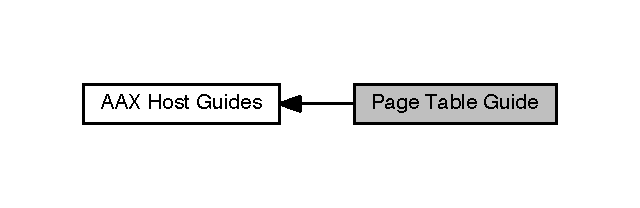
\includegraphics[width=307pt]{a00363}
\end{center}
\end{figure}
